% **************************************************************************************************************
% A Classic Thesis Style
% An Homage to The Elements of Typographic Style
%
% Copyright (C) 2012 Andr\'e Miede http://www.miede.de
%
% If you like the style then I would appreciate a postcard. My address
% can be found in the file ClassicThesis.pdf. A collection of the
% postcards I received so far is available online at
% http://postcards.miede.de
%
% License:
% This program is free software; you can redistribute it and/or modify
% it under the terms of the GNU General Public License as published by
% the Free Software Foundation; either version 2 of the License, or
% (at your option) any later version.
%
% This program is distributed in the hope that it will be useful,
% but WITHOUT ANY WARRANTY; without even the implied warranty of
% MERCHANTABILITY or FITNESS FOR A PARTICULAR PURPOSE.  See the
% GNU General Public License for more details.
%
% You should have received a copy of the GNU General Public License
% along with this program; see the file COPYING.  If not, write to
% the Free Software Foundation, Inc., 59 Temple Place - Suite 330,
% Boston, MA 02111-1307, USA.
%
% **************************************************************************************************************
% Note:
%    * You must not use "u etc. in strings/commands that will be spaced out (use \"u or real umlauts instead)
%    * New enumeration (small caps): \begin{aenumerate} \end{aenumerate}
%    * For margin notes: \marginpar or \graffito{}
%    * Do not use bold fonts in this style, it is designed around them
%    * Use tables as in the examples
%    * See classicthesis-preamble.sty for useful commands
% **************************************************************************************************************
\documentclass[ openright,titlepage,numbers=noenddot,headinclude,%1headlines,% letterpaper a4paper
                footinclude=true,cleardoublepage=empty,abstractoff, % <--- obsolete, remove (todo)
                BCOR=5mm,paper=a4,fontsize=11pt,%11pt,a4paper,%
                ngerman,american,openany
                ]{scrreprt}

%********************************************************************
% Note: Make all your adjustments in here
%*******************************************************
% ****************************************************************************************************
% classicthesis-config.tex
% formerly known as loadpackages.sty, classicthesis-ldpkg.sty, and classicthesis-preamble.sty
% Use it at the beginning of your ClassicThesis.tex, or as a LaTeX Preamble
% in your ClassicThesis.{tex,lyx} with % ****************************************************************************************************
% classicthesis-config.tex
% formerly known as loadpackages.sty, classicthesis-ldpkg.sty, and classicthesis-preamble.sty
% Use it at the beginning of your ClassicThesis.tex, or as a LaTeX Preamble
% in your ClassicThesis.{tex,lyx} with % ****************************************************************************************************
% classicthesis-config.tex
% formerly known as loadpackages.sty, classicthesis-ldpkg.sty, and classicthesis-preamble.sty
% Use it at the beginning of your ClassicThesis.tex, or as a LaTeX Preamble
% in your ClassicThesis.{tex,lyx} with \input{classicthesis-config}
% ****************************************************************************************************
% If you like the classicthesis, then I would appreciate a postcard.
% My address can be found in the file ClassicThesis.pdf. A collection
% of the postcards I received so far is available online at
% http://postcards.miede.de
% ****************************************************************************************************

% ****************************************************************************************************
% 1. Configure classicthesis for your needs here, e.g., remove "drafting" below
% in order to deactivate the time-stamp on the pages
% ****************************************************************************************************
\PassOptionsToPackage{eulerchapternumbers,listings,drafting,%
				 pdfspacing,%floatperchapter,%linedheaders,%
				 subfig,beramono,eulermath,parts}{classicthesis}
% ********************************************************************
% Available options for classicthesis.sty
% (see ClassicThesis.pdf for more information):
% drafting
% parts nochapters linedheaders
% eulerchapternumbers beramono eulermath pdfspacing minionprospacing
% tocaligned dottedtoc manychapters
% listings floatperchapter subfig
% ********************************************************************

% ********************************************************************
% Triggers for this config
% ********************************************************************
\usepackage{ifthen}
\newboolean{enable-backrefs} % enable backrefs in the bibliography
\setboolean{enable-backrefs}{false} % true false
% ****************************************************************************************************


% ****************************************************************************************************
% 2. Personal data and user ad-hoc commands
% ****************************************************************************************************
\newcommand{\myTitle}{Assisted headhunting\xspace}
\newcommand{\mySubtitle}{Pre-selecting job candidates through data analysis\xspace}
\newcommand{\myDegree}{\xspace}
\newcommand{\myName}{Felix Wolff\xspace}
\newcommand{\myProf}{Prof. Dr. Christoph Meinel\xspace}
\newcommand{\mySupervisor}{Philipp Berger, Patrick Hennig\xspace}
\newcommand{\myFaculty}{Internet- und WWW-Technologien\xspace}
\newcommand{\myDepartment}{Bachelorproject M1\xspace}
\newcommand{\myUni}{Hasso Plattner Institut\xspace}
\newcommand{\myLocation}{Potsdam\xspace}
\newcommand{\myTime}{July 2014\xspace}
\newcommand{\myVersion}{version 0.1\xspace}

% ********************************************************************
% Setup, finetuning, and useful commands
% ********************************************************************
\newcounter{dummy} % necessary for correct hyperlinks (to index, bib, etc.)
\newlength{\abcd} % for ab..z string length calculation
\providecommand{\mLyX}{L\kern-.1667em\lower.25em\hbox{Y}\kern-.125emX\@}
\newcommand{\ie}{i.\,e.}
\newcommand{\Ie}{I.\,e.}
\newcommand{\eg}{e.\,g.}
\newcommand{\Eg}{E.\,g.}
% ****************************************************************************************************


% ****************************************************************************************************
% 3. Loading some handy packages
% ****************************************************************************************************
% ********************************************************************
% Packages with options that might require adjustments
% ********************************************************************
\PassOptionsToPackage{latin9}{inputenc}	% latin9 (ISO-8859-9) = latin1+"Euro sign"
 \usepackage{inputenc}

%\PassOptionsToPackage{ngerman,american}{babel}   % change this to your language(s)
% Spanish languages need extra options in order to work with this template
%\PassOptionsToPackage{spanish,es-lcroman}{babel}
 \usepackage{babel}

\PassOptionsToPackage{square,numbers}{natbib}
 \usepackage{natbib}

\PassOptionsToPackage{fleqn}{amsmath}		% math environments and more by the AMS
 \usepackage{amsmath}

% ********************************************************************
% General useful packages
% ********************************************************************
\PassOptionsToPackage{T1}{fontenc} % T2A for cyrillics
	\usepackage{fontenc}
\usepackage{textcomp} % fix warning with missing font shapes
\usepackage{scrhack} % fix warnings when using KOMA with listings package
\usepackage{xspace} % to get the spacing after macros right
\usepackage{mparhack} % get marginpar right
\usepackage{fixltx2e} % fixes some LaTeX stuff
\PassOptionsToPackage{printonlyused,smaller}{acronym}
	\usepackage{acronym} % nice macros for handling all acronyms in the thesis
%\renewcommand*{\acsfont}[1]{\textssc{#1}} % for MinionPro
%\renewcommand{\bflabel}[1]{{#1}\hfill} % fix the list of acronyms
% ****************************************************************************************************


% ****************************************************************************************************
% 4. Setup floats: tables, (sub)figures, and captions
% ****************************************************************************************************
\usepackage{tabularx} % better tables
	\setlength{\extrarowheight}{3pt} % increase table row height
\newcommand{\tableheadline}[1]{\multicolumn{1}{c}{\spacedlowsmallcaps{#1}}}
\newcommand{\myfloatalign}{\centering} % to be used with each float for alignment
\usepackage{caption}
\captionsetup{format=hang,font=small}
\usepackage{subfig}
% ****************************************************************************************************


% ****************************************************************************************************
% 5. Setup code listings
% ****************************************************************************************************
\usepackage{listings}
%\lstset{emph={trueIndex,root},emphstyle=\color{BlueViolet}}%\underbar} % for special keywords
\lstset{language=[LaTeX]Tex,%C++,
    keywordstyle=\color{RoyalBlue},%\bfseries,
    basicstyle=\small\ttfamily,
    %identifierstyle=\color{NavyBlue},
    commentstyle=\color{Green}\ttfamily,
    stringstyle=\rmfamily,
    numbers=none,%left,%
    numberstyle=\scriptsize,%\tiny
    stepnumber=5,
    numbersep=8pt,
    showstringspaces=false,
    breaklines=true,
    frameround=ftff,
    frame=single,
    belowcaptionskip=.75\baselineskip
    %frame=L
}
% ****************************************************************************************************


% ****************************************************************************************************
% 6. PDFLaTeX, hyperreferences and citation backreferences
% ****************************************************************************************************
% ********************************************************************
% Using PDFLaTeX
% ********************************************************************
\PassOptionsToPackage{pdftex,hyperfootnotes=false,pdfpagelabels}{hyperref}
	\usepackage{hyperref}  % backref linktocpage pagebackref
\pdfcompresslevel=9
\pdfadjustspacing=1
\PassOptionsToPackage{pdftex}{graphicx}
	\usepackage{graphicx}

% ********************************************************************
% Setup the style of the backrefs from the bibliography
% (translate the options to any language you use)
% ********************************************************************
\newcommand{\backrefnotcitedstring}{\relax}%(Not cited.)
\newcommand{\backrefcitedsinglestring}[1]{(Cited on page~#1.)}
\newcommand{\backrefcitedmultistring}[1]{(Cited on pages~#1.)}
\ifthenelse{\boolean{enable-backrefs}}%
{%
		\PassOptionsToPackage{hyperpageref}{backref}
		\usepackage{backref} % to be loaded after hyperref package
		   \renewcommand{\backreftwosep}{ and~} % separate 2 pages
		   \renewcommand{\backreflastsep}{, and~} % separate last of longer list
		   \renewcommand*{\backref}[1]{}  % disable standard
		   \renewcommand*{\backrefalt}[4]{% detailed backref
		      \ifcase #1 %
		         \backrefnotcitedstring%
		      \or%
		         \backrefcitedsinglestring{#2}%
		      \else%
		         \backrefcitedmultistring{#2}%
		      \fi}%
}{\relax}

% ********************************************************************
% Hyperreferences
% ********************************************************************
\hypersetup{%
    %draft,	% = no hyperlinking at all (useful in b/w printouts)
    colorlinks=true, linktocpage=true, pdfstartpage=3, pdfstartview=FitV,%
    % uncomment the following line if you want to have black links (e.g., for printing)
    %colorlinks=false, linktocpage=false, pdfborder={0 0 0}, pdfstartpage=3, pdfstartview=FitV,%
    breaklinks=true, pdfpagemode=UseNone, pageanchor=true, pdfpagemode=UseOutlines,%
    plainpages=false, bookmarksnumbered, bookmarksopen=true, bookmarksopenlevel=1,%
    hypertexnames=true, pdfhighlight=/O,%nesting=true,%frenchlinks,%
    urlcolor=webbrown, linkcolor=RoyalBlue, citecolor=webgreen, %pagecolor=RoyalBlue,%
    %urlcolor=Black, linkcolor=Black, citecolor=Black, %pagecolor=Black,%
    pdftitle={\myTitle},%
    pdfauthor={\textcopyright\ \myName, \myUni, \myFaculty},%
    pdfsubject={},%
    pdfkeywords={},%
    pdfcreator={pdfLaTeX},%
    pdfproducer={LaTeX with hyperref and classicthesis}%
}

% ********************************************************************
% Setup autoreferences
% ********************************************************************
% There are some issues regarding autorefnames
% http://www.ureader.de/msg/136221647.aspx
% http://www.tex.ac.uk/cgi-bin/texfaq2html?label=latexwords
% you have to redefine the makros for the
% language you use, e.g., american, ngerman
% (as chosen when loading babel/AtBeginDocument)
% ********************************************************************
\makeatletter
\@ifpackageloaded{babel}%
    {%
       \addto\extrasamerican{%
					\renewcommand*{\figureautorefname}{Figure}%
					\renewcommand*{\tableautorefname}{Table}%
					\renewcommand*{\partautorefname}{Part}%
					\renewcommand*{\chapterautorefname}{Chapter}%
					\renewcommand*{\sectionautorefname}{Section}%
					\renewcommand*{\subsectionautorefname}{Section}%
					\renewcommand*{\subsubsectionautorefname}{Section}%
				}%
       \addto\extrasngerman{%
					\renewcommand*{\paragraphautorefname}{Absatz}%
					\renewcommand*{\subparagraphautorefname}{Unterabsatz}%
					\renewcommand*{\footnoteautorefname}{Fu\"snote}%
					\renewcommand*{\FancyVerbLineautorefname}{Zeile}%
					\renewcommand*{\theoremautorefname}{Theorem}%
					\renewcommand*{\appendixautorefname}{Anhang}%
					\renewcommand*{\equationautorefname}{Gleichung}%
					\renewcommand*{\itemautorefname}{Punkt}%
				}%
			% Fix to getting autorefs for subfigures right (thanks to Belinda Vogt for changing the definition)
			\providecommand{\subfigureautorefname}{\figureautorefname}%
    }{\relax}
\makeatother


% ****************************************************************************************************
% 7. Last calls before the bar closes
% ****************************************************************************************************
% ********************************************************************
% Development Stuff
% ********************************************************************
\listfiles
%\PassOptionsToPackage{l2tabu,orthodox,abort}{nag}
%	\usepackage{nag}
%\PassOptionsToPackage{warning, all}{onlyamsmath}
%	\usepackage{onlyamsmath}

% ********************************************************************
% Last, but not least...
% ********************************************************************
\usepackage{classicthesis}
% ****************************************************************************************************


% ****************************************************************************************************
% 8. Further adjustments (experimental)
% ****************************************************************************************************
% ********************************************************************
% Changing the text area
% ********************************************************************
%\linespread{1.05} % a bit more for Palatino
%\areaset[current]{312pt}{761pt} % 686 (factor 2.2) + 33 head + 42 head \the\footskip
%\setlength{\marginparwidth}{7em}%
%\setlength{\marginparsep}{2em}%

% ********************************************************************
% Using different fonts
% ********************************************************************
%\usepackage[oldstylenums]{kpfonts} % oldstyle notextcomp
%\usepackage[osf]{libertine}
%\usepackage{hfoldsty} % Computer Modern with osf
%\usepackage[light,condensed,math]{iwona}
%\renewcommand{\sfdefault}{iwona}
%\usepackage{lmodern} % <-- no osf support :-(
%\usepackage[urw-garamond]{mathdesign} <-- no osf support :-(
% ****************************************************************************************************

% ****************************************************************************************************
% If you like the classicthesis, then I would appreciate a postcard.
% My address can be found in the file ClassicThesis.pdf. A collection
% of the postcards I received so far is available online at
% http://postcards.miede.de
% ****************************************************************************************************

% ****************************************************************************************************
% 1. Configure classicthesis for your needs here, e.g., remove "drafting" below
% in order to deactivate the time-stamp on the pages
% ****************************************************************************************************
\PassOptionsToPackage{eulerchapternumbers,listings,drafting,%
				 pdfspacing,%floatperchapter,%linedheaders,%
				 subfig,beramono,eulermath,parts}{classicthesis}
% ********************************************************************
% Available options for classicthesis.sty
% (see ClassicThesis.pdf for more information):
% drafting
% parts nochapters linedheaders
% eulerchapternumbers beramono eulermath pdfspacing minionprospacing
% tocaligned dottedtoc manychapters
% listings floatperchapter subfig
% ********************************************************************

% ********************************************************************
% Triggers for this config
% ********************************************************************
\usepackage{ifthen}
\newboolean{enable-backrefs} % enable backrefs in the bibliography
\setboolean{enable-backrefs}{false} % true false
% ****************************************************************************************************


% ****************************************************************************************************
% 2. Personal data and user ad-hoc commands
% ****************************************************************************************************
\newcommand{\myTitle}{Assisted headhunting\xspace}
\newcommand{\mySubtitle}{Pre-selecting job candidates through data analysis\xspace}
\newcommand{\myDegree}{\xspace}
\newcommand{\myName}{Felix Wolff\xspace}
\newcommand{\myProf}{Prof. Dr. Christoph Meinel\xspace}
\newcommand{\mySupervisor}{Philipp Berger, Patrick Hennig\xspace}
\newcommand{\myFaculty}{Internet- und WWW-Technologien\xspace}
\newcommand{\myDepartment}{Bachelorproject M1\xspace}
\newcommand{\myUni}{Hasso Plattner Institut\xspace}
\newcommand{\myLocation}{Potsdam\xspace}
\newcommand{\myTime}{July 2014\xspace}
\newcommand{\myVersion}{version 0.1\xspace}

% ********************************************************************
% Setup, finetuning, and useful commands
% ********************************************************************
\newcounter{dummy} % necessary for correct hyperlinks (to index, bib, etc.)
\newlength{\abcd} % for ab..z string length calculation
\providecommand{\mLyX}{L\kern-.1667em\lower.25em\hbox{Y}\kern-.125emX\@}
\newcommand{\ie}{i.\,e.}
\newcommand{\Ie}{I.\,e.}
\newcommand{\eg}{e.\,g.}
\newcommand{\Eg}{E.\,g.}
% ****************************************************************************************************


% ****************************************************************************************************
% 3. Loading some handy packages
% ****************************************************************************************************
% ********************************************************************
% Packages with options that might require adjustments
% ********************************************************************
\PassOptionsToPackage{latin9}{inputenc}	% latin9 (ISO-8859-9) = latin1+"Euro sign"
 \usepackage{inputenc}

%\PassOptionsToPackage{ngerman,american}{babel}   % change this to your language(s)
% Spanish languages need extra options in order to work with this template
%\PassOptionsToPackage{spanish,es-lcroman}{babel}
 \usepackage{babel}

\PassOptionsToPackage{square,numbers}{natbib}
 \usepackage{natbib}

\PassOptionsToPackage{fleqn}{amsmath}		% math environments and more by the AMS
 \usepackage{amsmath}

% ********************************************************************
% General useful packages
% ********************************************************************
\PassOptionsToPackage{T1}{fontenc} % T2A for cyrillics
	\usepackage{fontenc}
\usepackage{textcomp} % fix warning with missing font shapes
\usepackage{scrhack} % fix warnings when using KOMA with listings package
\usepackage{xspace} % to get the spacing after macros right
\usepackage{mparhack} % get marginpar right
\usepackage{fixltx2e} % fixes some LaTeX stuff
\PassOptionsToPackage{printonlyused,smaller}{acronym}
	\usepackage{acronym} % nice macros for handling all acronyms in the thesis
%\renewcommand*{\acsfont}[1]{\textssc{#1}} % for MinionPro
%\renewcommand{\bflabel}[1]{{#1}\hfill} % fix the list of acronyms
% ****************************************************************************************************


% ****************************************************************************************************
% 4. Setup floats: tables, (sub)figures, and captions
% ****************************************************************************************************
\usepackage{tabularx} % better tables
	\setlength{\extrarowheight}{3pt} % increase table row height
\newcommand{\tableheadline}[1]{\multicolumn{1}{c}{\spacedlowsmallcaps{#1}}}
\newcommand{\myfloatalign}{\centering} % to be used with each float for alignment
\usepackage{caption}
\captionsetup{format=hang,font=small}
\usepackage{subfig}
% ****************************************************************************************************


% ****************************************************************************************************
% 5. Setup code listings
% ****************************************************************************************************
\usepackage{listings}
%\lstset{emph={trueIndex,root},emphstyle=\color{BlueViolet}}%\underbar} % for special keywords
\lstset{language=[LaTeX]Tex,%C++,
    keywordstyle=\color{RoyalBlue},%\bfseries,
    basicstyle=\small\ttfamily,
    %identifierstyle=\color{NavyBlue},
    commentstyle=\color{Green}\ttfamily,
    stringstyle=\rmfamily,
    numbers=none,%left,%
    numberstyle=\scriptsize,%\tiny
    stepnumber=5,
    numbersep=8pt,
    showstringspaces=false,
    breaklines=true,
    frameround=ftff,
    frame=single,
    belowcaptionskip=.75\baselineskip
    %frame=L
}
% ****************************************************************************************************


% ****************************************************************************************************
% 6. PDFLaTeX, hyperreferences and citation backreferences
% ****************************************************************************************************
% ********************************************************************
% Using PDFLaTeX
% ********************************************************************
\PassOptionsToPackage{pdftex,hyperfootnotes=false,pdfpagelabels}{hyperref}
	\usepackage{hyperref}  % backref linktocpage pagebackref
\pdfcompresslevel=9
\pdfadjustspacing=1
\PassOptionsToPackage{pdftex}{graphicx}
	\usepackage{graphicx}

% ********************************************************************
% Setup the style of the backrefs from the bibliography
% (translate the options to any language you use)
% ********************************************************************
\newcommand{\backrefnotcitedstring}{\relax}%(Not cited.)
\newcommand{\backrefcitedsinglestring}[1]{(Cited on page~#1.)}
\newcommand{\backrefcitedmultistring}[1]{(Cited on pages~#1.)}
\ifthenelse{\boolean{enable-backrefs}}%
{%
		\PassOptionsToPackage{hyperpageref}{backref}
		\usepackage{backref} % to be loaded after hyperref package
		   \renewcommand{\backreftwosep}{ and~} % separate 2 pages
		   \renewcommand{\backreflastsep}{, and~} % separate last of longer list
		   \renewcommand*{\backref}[1]{}  % disable standard
		   \renewcommand*{\backrefalt}[4]{% detailed backref
		      \ifcase #1 %
		         \backrefnotcitedstring%
		      \or%
		         \backrefcitedsinglestring{#2}%
		      \else%
		         \backrefcitedmultistring{#2}%
		      \fi}%
}{\relax}

% ********************************************************************
% Hyperreferences
% ********************************************************************
\hypersetup{%
    %draft,	% = no hyperlinking at all (useful in b/w printouts)
    colorlinks=true, linktocpage=true, pdfstartpage=3, pdfstartview=FitV,%
    % uncomment the following line if you want to have black links (e.g., for printing)
    %colorlinks=false, linktocpage=false, pdfborder={0 0 0}, pdfstartpage=3, pdfstartview=FitV,%
    breaklinks=true, pdfpagemode=UseNone, pageanchor=true, pdfpagemode=UseOutlines,%
    plainpages=false, bookmarksnumbered, bookmarksopen=true, bookmarksopenlevel=1,%
    hypertexnames=true, pdfhighlight=/O,%nesting=true,%frenchlinks,%
    urlcolor=webbrown, linkcolor=RoyalBlue, citecolor=webgreen, %pagecolor=RoyalBlue,%
    %urlcolor=Black, linkcolor=Black, citecolor=Black, %pagecolor=Black,%
    pdftitle={\myTitle},%
    pdfauthor={\textcopyright\ \myName, \myUni, \myFaculty},%
    pdfsubject={},%
    pdfkeywords={},%
    pdfcreator={pdfLaTeX},%
    pdfproducer={LaTeX with hyperref and classicthesis}%
}

% ********************************************************************
% Setup autoreferences
% ********************************************************************
% There are some issues regarding autorefnames
% http://www.ureader.de/msg/136221647.aspx
% http://www.tex.ac.uk/cgi-bin/texfaq2html?label=latexwords
% you have to redefine the makros for the
% language you use, e.g., american, ngerman
% (as chosen when loading babel/AtBeginDocument)
% ********************************************************************
\makeatletter
\@ifpackageloaded{babel}%
    {%
       \addto\extrasamerican{%
					\renewcommand*{\figureautorefname}{Figure}%
					\renewcommand*{\tableautorefname}{Table}%
					\renewcommand*{\partautorefname}{Part}%
					\renewcommand*{\chapterautorefname}{Chapter}%
					\renewcommand*{\sectionautorefname}{Section}%
					\renewcommand*{\subsectionautorefname}{Section}%
					\renewcommand*{\subsubsectionautorefname}{Section}%
				}%
       \addto\extrasngerman{%
					\renewcommand*{\paragraphautorefname}{Absatz}%
					\renewcommand*{\subparagraphautorefname}{Unterabsatz}%
					\renewcommand*{\footnoteautorefname}{Fu\"snote}%
					\renewcommand*{\FancyVerbLineautorefname}{Zeile}%
					\renewcommand*{\theoremautorefname}{Theorem}%
					\renewcommand*{\appendixautorefname}{Anhang}%
					\renewcommand*{\equationautorefname}{Gleichung}%
					\renewcommand*{\itemautorefname}{Punkt}%
				}%
			% Fix to getting autorefs for subfigures right (thanks to Belinda Vogt for changing the definition)
			\providecommand{\subfigureautorefname}{\figureautorefname}%
    }{\relax}
\makeatother


% ****************************************************************************************************
% 7. Last calls before the bar closes
% ****************************************************************************************************
% ********************************************************************
% Development Stuff
% ********************************************************************
\listfiles
%\PassOptionsToPackage{l2tabu,orthodox,abort}{nag}
%	\usepackage{nag}
%\PassOptionsToPackage{warning, all}{onlyamsmath}
%	\usepackage{onlyamsmath}

% ********************************************************************
% Last, but not least...
% ********************************************************************
\usepackage{classicthesis}
% ****************************************************************************************************


% ****************************************************************************************************
% 8. Further adjustments (experimental)
% ****************************************************************************************************
% ********************************************************************
% Changing the text area
% ********************************************************************
%\linespread{1.05} % a bit more for Palatino
%\areaset[current]{312pt}{761pt} % 686 (factor 2.2) + 33 head + 42 head \the\footskip
%\setlength{\marginparwidth}{7em}%
%\setlength{\marginparsep}{2em}%

% ********************************************************************
% Using different fonts
% ********************************************************************
%\usepackage[oldstylenums]{kpfonts} % oldstyle notextcomp
%\usepackage[osf]{libertine}
%\usepackage{hfoldsty} % Computer Modern with osf
%\usepackage[light,condensed,math]{iwona}
%\renewcommand{\sfdefault}{iwona}
%\usepackage{lmodern} % <-- no osf support :-(
%\usepackage[urw-garamond]{mathdesign} <-- no osf support :-(
% ****************************************************************************************************

% ****************************************************************************************************
% If you like the classicthesis, then I would appreciate a postcard.
% My address can be found in the file ClassicThesis.pdf. A collection
% of the postcards I received so far is available online at
% http://postcards.miede.de
% ****************************************************************************************************

% ****************************************************************************************************
% 1. Configure classicthesis for your needs here, e.g., remove "drafting" below
% in order to deactivate the time-stamp on the pages
% ****************************************************************************************************
\PassOptionsToPackage{eulerchapternumbers,listings,drafting,%
				 pdfspacing,%floatperchapter,%linedheaders,%
				 subfig,beramono,eulermath,parts}{classicthesis}
% ********************************************************************
% Available options for classicthesis.sty
% (see ClassicThesis.pdf for more information):
% drafting
% parts nochapters linedheaders
% eulerchapternumbers beramono eulermath pdfspacing minionprospacing
% tocaligned dottedtoc manychapters
% listings floatperchapter subfig
% ********************************************************************

% ********************************************************************
% Triggers for this config
% ********************************************************************
\usepackage{ifthen}
\newboolean{enable-backrefs} % enable backrefs in the bibliography
\setboolean{enable-backrefs}{false} % true false
% ****************************************************************************************************


% ****************************************************************************************************
% 2. Personal data and user ad-hoc commands
% ****************************************************************************************************
\newcommand{\myTitle}{Assisted headhunting\xspace}
\newcommand{\mySubtitle}{Pre-selecting job candidates through data analysis\xspace}
\newcommand{\myDegree}{\xspace}
\newcommand{\myName}{Felix Wolff\xspace}
\newcommand{\myProf}{Prof. Dr. Christoph Meinel\xspace}
\newcommand{\mySupervisor}{Philipp Berger, Patrick Hennig\xspace}
\newcommand{\myFaculty}{Internet- und WWW-Technologien\xspace}
\newcommand{\myDepartment}{Bachelorproject M1\xspace}
\newcommand{\myUni}{Hasso Plattner Institut\xspace}
\newcommand{\myLocation}{Potsdam\xspace}
\newcommand{\myTime}{July 2014\xspace}
\newcommand{\myVersion}{version 0.1\xspace}

% ********************************************************************
% Setup, finetuning, and useful commands
% ********************************************************************
\newcounter{dummy} % necessary for correct hyperlinks (to index, bib, etc.)
\newlength{\abcd} % for ab..z string length calculation
\providecommand{\mLyX}{L\kern-.1667em\lower.25em\hbox{Y}\kern-.125emX\@}
\newcommand{\ie}{i.\,e.}
\newcommand{\Ie}{I.\,e.}
\newcommand{\eg}{e.\,g.}
\newcommand{\Eg}{E.\,g.}
% ****************************************************************************************************


% ****************************************************************************************************
% 3. Loading some handy packages
% ****************************************************************************************************
% ********************************************************************
% Packages with options that might require adjustments
% ********************************************************************
\PassOptionsToPackage{latin9}{inputenc}	% latin9 (ISO-8859-9) = latin1+"Euro sign"
 \usepackage{inputenc}

%\PassOptionsToPackage{ngerman,american}{babel}   % change this to your language(s)
% Spanish languages need extra options in order to work with this template
%\PassOptionsToPackage{spanish,es-lcroman}{babel}
 \usepackage{babel}

\PassOptionsToPackage{square,numbers}{natbib}
 \usepackage{natbib}

\PassOptionsToPackage{fleqn}{amsmath}		% math environments and more by the AMS
 \usepackage{amsmath}

% ********************************************************************
% General useful packages
% ********************************************************************
\PassOptionsToPackage{T1}{fontenc} % T2A for cyrillics
	\usepackage{fontenc}
\usepackage{textcomp} % fix warning with missing font shapes
\usepackage{scrhack} % fix warnings when using KOMA with listings package
\usepackage{xspace} % to get the spacing after macros right
\usepackage{mparhack} % get marginpar right
\usepackage{fixltx2e} % fixes some LaTeX stuff
\PassOptionsToPackage{printonlyused,smaller}{acronym}
	\usepackage{acronym} % nice macros for handling all acronyms in the thesis
%\renewcommand*{\acsfont}[1]{\textssc{#1}} % for MinionPro
%\renewcommand{\bflabel}[1]{{#1}\hfill} % fix the list of acronyms
% ****************************************************************************************************


% ****************************************************************************************************
% 4. Setup floats: tables, (sub)figures, and captions
% ****************************************************************************************************
\usepackage{tabularx} % better tables
	\setlength{\extrarowheight}{3pt} % increase table row height
\newcommand{\tableheadline}[1]{\multicolumn{1}{c}{\spacedlowsmallcaps{#1}}}
\newcommand{\myfloatalign}{\centering} % to be used with each float for alignment
\usepackage{caption}
\captionsetup{format=hang,font=small}
\usepackage{subfig}
% ****************************************************************************************************


% ****************************************************************************************************
% 5. Setup code listings
% ****************************************************************************************************
\usepackage{listings}
%\lstset{emph={trueIndex,root},emphstyle=\color{BlueViolet}}%\underbar} % for special keywords
\lstset{language=[LaTeX]Tex,%C++,
    keywordstyle=\color{RoyalBlue},%\bfseries,
    basicstyle=\small\ttfamily,
    %identifierstyle=\color{NavyBlue},
    commentstyle=\color{Green}\ttfamily,
    stringstyle=\rmfamily,
    numbers=none,%left,%
    numberstyle=\scriptsize,%\tiny
    stepnumber=5,
    numbersep=8pt,
    showstringspaces=false,
    breaklines=true,
    frameround=ftff,
    frame=single,
    belowcaptionskip=.75\baselineskip
    %frame=L
}
% ****************************************************************************************************


% ****************************************************************************************************
% 6. PDFLaTeX, hyperreferences and citation backreferences
% ****************************************************************************************************
% ********************************************************************
% Using PDFLaTeX
% ********************************************************************
\PassOptionsToPackage{pdftex,hyperfootnotes=false,pdfpagelabels}{hyperref}
	\usepackage{hyperref}  % backref linktocpage pagebackref
\pdfcompresslevel=9
\pdfadjustspacing=1
\PassOptionsToPackage{pdftex}{graphicx}
	\usepackage{graphicx}

% ********************************************************************
% Setup the style of the backrefs from the bibliography
% (translate the options to any language you use)
% ********************************************************************
\newcommand{\backrefnotcitedstring}{\relax}%(Not cited.)
\newcommand{\backrefcitedsinglestring}[1]{(Cited on page~#1.)}
\newcommand{\backrefcitedmultistring}[1]{(Cited on pages~#1.)}
\ifthenelse{\boolean{enable-backrefs}}%
{%
		\PassOptionsToPackage{hyperpageref}{backref}
		\usepackage{backref} % to be loaded after hyperref package
		   \renewcommand{\backreftwosep}{ and~} % separate 2 pages
		   \renewcommand{\backreflastsep}{, and~} % separate last of longer list
		   \renewcommand*{\backref}[1]{}  % disable standard
		   \renewcommand*{\backrefalt}[4]{% detailed backref
		      \ifcase #1 %
		         \backrefnotcitedstring%
		      \or%
		         \backrefcitedsinglestring{#2}%
		      \else%
		         \backrefcitedmultistring{#2}%
		      \fi}%
}{\relax}

% ********************************************************************
% Hyperreferences
% ********************************************************************
\hypersetup{%
    %draft,	% = no hyperlinking at all (useful in b/w printouts)
    colorlinks=true, linktocpage=true, pdfstartpage=3, pdfstartview=FitV,%
    % uncomment the following line if you want to have black links (e.g., for printing)
    %colorlinks=false, linktocpage=false, pdfborder={0 0 0}, pdfstartpage=3, pdfstartview=FitV,%
    breaklinks=true, pdfpagemode=UseNone, pageanchor=true, pdfpagemode=UseOutlines,%
    plainpages=false, bookmarksnumbered, bookmarksopen=true, bookmarksopenlevel=1,%
    hypertexnames=true, pdfhighlight=/O,%nesting=true,%frenchlinks,%
    urlcolor=webbrown, linkcolor=RoyalBlue, citecolor=webgreen, %pagecolor=RoyalBlue,%
    %urlcolor=Black, linkcolor=Black, citecolor=Black, %pagecolor=Black,%
    pdftitle={\myTitle},%
    pdfauthor={\textcopyright\ \myName, \myUni, \myFaculty},%
    pdfsubject={},%
    pdfkeywords={},%
    pdfcreator={pdfLaTeX},%
    pdfproducer={LaTeX with hyperref and classicthesis}%
}

% ********************************************************************
% Setup autoreferences
% ********************************************************************
% There are some issues regarding autorefnames
% http://www.ureader.de/msg/136221647.aspx
% http://www.tex.ac.uk/cgi-bin/texfaq2html?label=latexwords
% you have to redefine the makros for the
% language you use, e.g., american, ngerman
% (as chosen when loading babel/AtBeginDocument)
% ********************************************************************
\makeatletter
\@ifpackageloaded{babel}%
    {%
       \addto\extrasamerican{%
					\renewcommand*{\figureautorefname}{Figure}%
					\renewcommand*{\tableautorefname}{Table}%
					\renewcommand*{\partautorefname}{Part}%
					\renewcommand*{\chapterautorefname}{Chapter}%
					\renewcommand*{\sectionautorefname}{Section}%
					\renewcommand*{\subsectionautorefname}{Section}%
					\renewcommand*{\subsubsectionautorefname}{Section}%
				}%
       \addto\extrasngerman{%
					\renewcommand*{\paragraphautorefname}{Absatz}%
					\renewcommand*{\subparagraphautorefname}{Unterabsatz}%
					\renewcommand*{\footnoteautorefname}{Fu\"snote}%
					\renewcommand*{\FancyVerbLineautorefname}{Zeile}%
					\renewcommand*{\theoremautorefname}{Theorem}%
					\renewcommand*{\appendixautorefname}{Anhang}%
					\renewcommand*{\equationautorefname}{Gleichung}%
					\renewcommand*{\itemautorefname}{Punkt}%
				}%
			% Fix to getting autorefs for subfigures right (thanks to Belinda Vogt for changing the definition)
			\providecommand{\subfigureautorefname}{\figureautorefname}%
    }{\relax}
\makeatother


% ****************************************************************************************************
% 7. Last calls before the bar closes
% ****************************************************************************************************
% ********************************************************************
% Development Stuff
% ********************************************************************
\listfiles
%\PassOptionsToPackage{l2tabu,orthodox,abort}{nag}
%	\usepackage{nag}
%\PassOptionsToPackage{warning, all}{onlyamsmath}
%	\usepackage{onlyamsmath}

% ********************************************************************
% Last, but not least...
% ********************************************************************
\usepackage{classicthesis}
% ****************************************************************************************************


% ****************************************************************************************************
% 8. Further adjustments (experimental)
% ****************************************************************************************************
% ********************************************************************
% Changing the text area
% ********************************************************************
%\linespread{1.05} % a bit more for Palatino
%\areaset[current]{312pt}{761pt} % 686 (factor 2.2) + 33 head + 42 head \the\footskip
%\setlength{\marginparwidth}{7em}%
%\setlength{\marginparsep}{2em}%

% ********************************************************************
% Using different fonts
% ********************************************************************
%\usepackage[oldstylenums]{kpfonts} % oldstyle notextcomp
%\usepackage[osf]{libertine}
%\usepackage{hfoldsty} % Computer Modern with osf
%\usepackage[light,condensed,math]{iwona}
%\renewcommand{\sfdefault}{iwona}
%\usepackage{lmodern} % <-- no osf support :-(
%\usepackage[urw-garamond]{mathdesign} <-- no osf support :-(
% ****************************************************************************************************


%********************************************************************
% Hyphenation
%*******************************************************
%\hyphenation{put special hyphenation here}

% ********************************************************************
% GO!GO!GO! MOVE IT!
%*******************************************************
\begin{document}
\frenchspacing
\raggedbottom
\selectlanguage{american} % american ngerman
%\renewcommand*{\bibname}{new name}
\renewcommand{\PrelimText}{}
%\setbibpreamble{}
\pagenumbering{roman}
\pagestyle{plain}
%********************************************************************
% Frontmatter
%*******************************************************
%%*******************************************************
% Little Dirty Titlepage
%*******************************************************
\thispagestyle{empty}
%\pdfbookmark[1]{Titel}{title}
%*******************************************************
\begin{center}
    \spacedlowsmallcaps{\myName} \\ \medskip                        

    \begingroup
        \color{Maroon}\spacedallcaps{\myTitle}
    \endgroup
\end{center}        

%*******************************************************
% Titlepage
%*******************************************************
\newenvironment{myepigraph}
  {\par\hfill
   \begin{tabular}{@{}r@{\hspace{13em}}}}
  {\end{tabular}\par\medskip}

\begin{titlepage}
	% if you want the titlepage to be centered, uncomment and fine-tune the line below (KOMA classes environment)
	\begin{addmargin}[-1cm]{-3cm}
    \begin{center}
        \hfill

        \vfill

        \begingroup
          \color{Maroon}\spacedallcaps{\myTitle} \\
          \color{Maroon}\spacedallcaps{\mySubtitle}\\[1em]
          \color{Black}\spacedlowsmallcaps{\myTitleGer}
          %\color{Black}\spacedlowsmallcaps{\mySubtitleGer}
          \\[3em]
        \endgroup

        {\color{Black}\spacedlowsmallcaps{\myName}\\
        \spacedlowsmallcaps{\myTime}}

        \hfill



        \vfill

        
\includegraphics[width=6cm]{gfx/logo.jpg} \\[2ex]
        \begin{myepigraph}
        \spacedlowsmallcaps{Supervised by}\\
        \myProf\\
        \mySupervisorA\\
        \mySupervisorB\\
        \spacedlowsmallcaps{\myFaculty}
        \end{myepigraph}

        \vfill

    \end{center}
  \end{addmargin}
\end{titlepage}
\thispagestyle{empty}

\hfill

\vfill

\noindent\myName: \textit{\myTitle,} \mySubtitle, %\myDegree, 
\textcopyright\ \myTime

%\bigskip
%
%\noindent\spacedlowsmallcaps{Supervisors}: \\
%\myProf \\
%\myOtherProf \\ 
%\mySupervisor
%
%\medskip
%
%\noindent\spacedlowsmallcaps{Location}: \\
%\myLocation
%
%\medskip
%
%\noindent\spacedlowsmallcaps{Time Frame}: \\
%\myTime

%\cleardoublepage%*******************************************************
% Dedication
%*******************************************************
\thispagestyle{empty}
%\phantomsection 
\refstepcounter{dummy}
\pdfbookmark[1]{Dedication}{Dedication}

\vspace*{3cm}

\begin{center}
    \emph{Ohana} means family. \\
    Family means nobody gets left behind, or forgotten. \\ \medskip
    --- Lilo \& Stitch    
\end{center}

\medskip

\begin{center}
    Dedicated to the loving memory of Rudolf Miede. \\ \smallskip
    1939\,--\,2005
\end{center}
%\cleardoublepage\input{frontbackmatter/foreword}
%*******************************************************
% Abstract
%*******************************************************
%\renewcommand{\abstractname}{Abstract}
\pdfbookmark[1]{Abstract}{Abstract}
\begingroup
\let\clearpage\relax
\let\cleardoublepage\relax
\let\cleardoublepage\relax

\chapter*{Abstract}
The volume of data produced on the Internet every day is growing rapidly. Especially social networks grow vastly and get filled with more and more content each second. The size of these networks has made them attractive as marketing platforms, but also for recruiting.

Specifically in the technology industry, talented colleagues are scarce and heavily sought after. While it is possible to go through social networks manually to hire top talent, it is not advisable, for a lot of data can not be covered due to lack of manpower. To harness greater processing power spanning over several social networks, a metric has been put together for comparing developers and matching them on to job opening requirements. For verifying it, a prototypical platform where recruiters can find developers by stating programming language requirements has been implemented.

The results of a comparison of the recommendations for a position with the opinions of the candidates about their suitability for it resulted in about 80\% accuracy. The metric is based on data from analyzed source code repositories and GitHub.


\vfill

\pdfbookmark[1]{Zusammenfassung}{Zusammenfassung}
\chapter*{Zusammenfassung}
Kurze Zusammenfassung des Inhaltes in deutscher Sprache\dots


\endgroup

\vfill
%\cleardoublepage%*******************************************************
% Publications
%*******************************************************
\pdfbookmark[1]{Publications}{publications}
\chapter*{Publications}
Some ideas and figures have appeared previously in the following publications:

\bigskip

\noindent Put your publications from the thesis here. The packages \texttt{multibib} or \texttt{bibtopic} etc. can be used to handle multiple different bibliographies in your document.
%%*******************************************************
% Acknowledgments
%*******************************************************
\pdfbookmark[1]{Acknowledgments}{acknowledgments}

\begin{flushright}{\slshape    
    We have seen that computer programming is an art, \\ 
    because it applies accumulated knowledge to the world, \\ 
    because it requires skill and ingenuity, and especially \\
    because it produces objects of beauty.} \\ \medskip
    --- \defcitealias{knuth:1974}{Donald E. Knuth}\citetalias{knuth:1974} \citep{knuth:1974}
\end{flushright}



\bigskip

\begingroup
\let\clearpage\relax
\let\cleardoublepage\relax
\let\cleardoublepage\relax
\chapter*{Acknowledgments}
Put your acknowledgments here.

Many thanks to everybody who already sent me a postcard!

Regarding the typography and other help, many thanks go to Marco 
Kuhlmann, Philipp Lehman, Lothar Schlesier, Jim Young, Lorenzo 
Pantieri and Enrico Gregorio\footnote{Members of GuIT (Gruppo 
Italiano Utilizzatori di \TeX\ e \LaTeX )}, J\"org Sommer, 
Joachim K\"ostler, Daniel Gottschlag, Denis Aydin, Paride 
Legovini, Steffen Prochnow, Nicolas Repp, Hinrich Harms, 
 Roland Winkler, J\"org Weber, 
 and the whole \LaTeX-community for support, ideas and 
 some great software.

\bigskip

\noindent\emph{Regarding \mLyX}: The \mLyX\ port was intially done by 
\emph{Nicholas Mariette} in March 2009 and continued by 
\emph{Ivo Pletikosi\'c} in 2011. Thank you very much for your 
work and the contributions to the original style.


\endgroup




\pagestyle{scrheadings}
%*******************************************************
% Table of Contents
%*******************************************************
%\phantomsection
\refstepcounter{dummy}
\pdfbookmark[1]{\contentsname}{tableofcontents}
\setcounter{tocdepth}{2} % <-- 2 includes up to subsections in the ToC
\setcounter{secnumdepth}{3} % <-- 3 numbers up to subsubsections
\manualmark
\markboth{\spacedlowsmallcaps{\contentsname}}{\spacedlowsmallcaps{\contentsname}}
\tableofcontents 
\automark[section]{chapter}
\renewcommand{\chaptermark}[1]{\markboth{\spacedlowsmallcaps{#1}}{\spacedlowsmallcaps{#1}}}
\renewcommand{\sectionmark}[1]{\markright{\thesection\enspace\spacedlowsmallcaps{#1}}}
%*******************************************************
% List of Figures and of the Tables
%*******************************************************
\clearpage

\begingroup 
    \let\clearpage\relax
    \let\cleardoublepage\relax
    \let\cleardoublepage\relax
    %*******************************************************
    % List of Figures
    %*******************************************************    
    %\phantomsection 
    \refstepcounter{dummy}
    %\addcontentsline{toc}{chapter}{\listfigurename}
    \pdfbookmark[1]{\listfigurename}{lof}
    \listoffigures

    \vspace*{8ex}

    %*******************************************************
    % List of Tables
    %*******************************************************
    %\phantomsection 
    \refstepcounter{dummy}
    %\addcontentsline{toc}{chapter}{\listtablename}
    \pdfbookmark[1]{\listtablename}{lot}
    \listoftables
        
    \vspace*{8ex}
%   \newpage
    
    %*******************************************************
    % List of Listings
    %*******************************************************      
	  %\phantomsection 
    \refstepcounter{dummy}
    %\addcontentsline{toc}{chapter}{\lstlistlistingname}
    \pdfbookmark[1]{\lstlistlistingname}{lol}
    \lstlistoflistings 

    \vspace*{8ex}
       
    %*******************************************************
    % Acronyms
    %*******************************************************
    %\phantomsection 
    \refstepcounter{dummy}
    \pdfbookmark[1]{Acronyms}{acronyms}
    \markboth{\spacedlowsmallcaps{Acronyms}}{\spacedlowsmallcaps{Acronyms}}
    \chapter*{Acronyms}
    \begin{acronym}[UML]
        \acro{DRY}{Don't Repeat Yourself}
        \acro{API}{Application Programming Interface}
        \acro{UML}{Unified Modeling Language}
    \end{acronym}                     
\endgroup

\cleardoublepage
%********************************************************************
% Mainmatter
%*******************************************************
\part{Thesis}
\pagenumbering{arabic}
%************************************************
\chapter{Introduction}\label{ch:introduction}
%************************************************
The war for talent is on. Coined at the beginning of the new
millenium, the term describes the increasing competition between companies
for skilled employees\footnote{\url{https://en.wikipedia.org/wiki/The_war_for_talent} | checked June 13, 2015}.

It is on, and it has never been more intense for technical experts\footnote{\url{http://tcrn.ch/1SXBKJl} | checked June 12, 2015}.
A perk that one company offers with one job is countered with another perk by
another company, and vice versa. Startup companies are being bought,
just for the acquirer to access much needed talent.
These so called "aquihires" often lead to an integration of the team into
the company and a cancellation of their old product\footnote{\url{http://bit.ly/1FuPbM7} | checked June 13, 2015}\footnote{\url{https://en.wikipedia.org/wiki/Acqui-hiring} | checked June 13, 2015}.
It even goes so far that companies bid for talent on online marketplaces, like
Hired\footnote{\url{https://hired.com} | checked June 19, 2015} or StartupCV\footnote{\url{https://www.startupcvs.com/} | checked June 19, 2015}.
\newline

Looking at programmers, a candidate for an opening is often put into test projects or given small programming tasks to solve. These should prove programming capability, and - given a successful completion - they are hired\footnote{\url{http://bit.ly/1LDNtvn} | checked June 13, 2015}. Both for developers and recruiters, this process feels slow and tedious, often resulting in frustration for the two. There should be ways of identifying such capabilities beforehand, and rather than conducting technical interviews or costly tests, we propose hereby a software-based method for matching technical talent on to technical requirements from job advertisements.

\section{Contribution}
In this thesis we will present a metric with which developers can be matched against job requirements and be ranked by suitability for it. The metric will build on top of data gathered from analyzed open source repositories. In order to verify it, we also present a platform on which recruiters can easily gain access to these software engineering talents. The recruiters can specifyn what kind of position they want to find candidates for, and will receive suggestions from the userbase that has registered with the application.

Github will be the only source of code in our case, but it has proven to be sufficiently large and well-frequented for our use case. The analysis metric has been constructed specifically for our use case, because to the best of our knowledge, no pre-existing method was suitable.

TODO - add platform image here

\section{Research Questions}\label{sec:research-questions}
To guide our research, we formulated two research questions:

\subsection{How can developer skills be measured?}\label{subsec:dev-skill-measurement}
Finding commonalities between job advertisements and skill profiles
requires some sort of reverence value. We argue that a measurement
metric needs be found.
In order to reduce the need for a lot of customization
on the advertisements and allow for  analysis of pre-existing data,
it should depend on data provided by most job opening descriptions.
\newline

All developers will be matched against the same job advertisements
and thus they all need to be measured using the same method.
The metric that has been derived from the advertisements will need to be
measured on each developer - provided he or she can provide the
necessary data. Thus the practicability of the metric depends largely on
the availability of measureable data.

\subsection{Can qualified candidates be found automatically?}\label{subsec:measurement-quality}
The metric allows developers to be ranked by suitability for the position.
The qualities of this ranking are ultimately determined by whether
or not the right candidates land at the top of it. This needs to be
verified with real world job candidates and the job opening descriptions
that they applied for

\section{Related Work}
Marlow et al.\cite{md:2013} have conducted an extensive study with about
200 participants, and found out that employers value
open source coder profiles greatly (page 4). The authors prove that developers are conscious of the fact
that their source code is public and thus try to deliver it with
great care. This is relevant for us for two reasons:
First, it proves that contribution to open source has a relevancy
in hiring and is awarded with recognition. And second, Marlows and Dabbishs
research hints at the fact that developers are trying hard to deliver very
good code, because they are aware of its publicity. Because we will use
exactly this code in our measurements, it is highly relevant that it be as good as its author can possibly write it.
Altogether their research has proven that both public sourcecode repositories
are relevant for making recruitment decisions and that open source developers
are aware of this fact and try to deliver their best.
\newline

The suitability of source code analysis for the identification of personal
skillsets has been demonstrated in the master thesis of Philipp Giese\cite{pg:2014}.
He built a framework called \textit{Analyzr}\footnote{\url{https://github.com/frontendphil/analyzr}}
that analyzes the complete history from a git or SVN source code repository.
Based on the code, different metrics are calculated, from which statements about
code complexity and refactoring needs can be derived. It is also possible
to make statements about developer capabilites and areas of expertise.
Thus, given a little context about the analyzed source code, it would possible
to say that \glqq Developer X is mainly a backend developer and the single maintainer of module Y\grqq.

Philipp's findings are supported by that of
Aftab Iqbal and Michael Hausenblas, who have analyzed different
source code repositories for common developers\cite{ih:2012}.
They have done so using relatively little local code analysis and relied
on on-the-fly analysis from retrieved RDF data. Their work
has made it possible to find out whether different open source projects shared developers
and contained useful methods of retrieving authors and eleminating duplicates
caused by different e-mail addresses, for example.
One of their primary sources of code was \textit{sourceforge}, a site that was
popular for open source code hosting before GitHub took its place.
Now, in 2015, sourceforge has more or less disappeared from the map of open
source developers and does not host a lot of projects of relevance anymore.

Vasilescu, Filkov and Serebrenik of TU Eindhoven have taken it further
and integrated developer-related information across several code forges
with crowdsourcing platforms such as StackOverflow\cite{vfs:2013}.
Their findings allow identifying active contributors on StackOverflow
as well as active developers on GitHub.
\newline

A japanese research group at the Kobe University in Tokio, seems
to display great interest in software analytics\cite{mn:2011}. Shinsuke Matsumoto and Masahide Nakamura
have built a web service that allowed the analysis of any SVN or git source code repository.
They were specifically interested in creating a platform for other researchers to
contribute their source code metrics to. The metrics are programming-language agnostic
and very general. Unfortunately the code was badly documented and if there was documentation
to be found, it was written in japanese. Matsumotos and Nakamuras paper
went into deep technical detail of the inner workings of their platform.
This knowledge was particularly helpful in the forming of an architecture for ours.

Matsumoto, Nakamura and Giese also hinted at several code metrics of historical
importance. They made use of McCabes Cyclomatic Complexity metric\cite{mc:1976}
and the Halstead complexity measures\cite{h:1977}.
The first provides a way for measuring computational complexity, which is
something that might hint at a clean design and a performant implementation.
Quite similarly, the latter focuses itself on static code as well, but with the
distinction of providing several metrics, like the presumable number of bugs and
a code difficulty indicator, all based on four small code-related numbers.
\newline

Algorithmically indentifying talent is something that has been tried by  any companies with recruiting at the core of their business model. For LinkedIn, the tools for recruiters that are fueled by this research are their main source of income\footnote{\url{http://tnw.co/1g20G4m} | checked June 29, 2015}. A startup called \textit{Work For Pie}\footnote{\url{http://www.workforpie.com/} | checked June 27, 2015} built a platform similar to ours and got acquired by the hiring platform GroupTalent. For this reason it was very hard to find information on the inner workings of the job recommendation system in production, which is why there is no comparison with their recommendation techniques in this thesis.

\section{Project background}
The basic concept of applying demand-based filtering can be traced back to a bachelor project at the Hasso-Plattner-Institute.

\marginpar{The bachelor project is a two-semester project at HPI, where 2-7 students work together on a large software system, often for an external partner. In the process, expertise for the bachelor thesis is gathered.}

In a world where cold calls have become outdated\cite{bh:2014}, social media platforms like facebook, Twitter, LinkedIn and Xing have grown to be important places for getting in touch with customers. 500 million tweets are sent on a single day on Twitter\footnote{\url{https://about.twitter.com/company} | checked June 29, 2015} alone. All platforms combined result in a huge marketing reach. To help covering most of this reach, the bachelor project implemented a system acquiring social media data, applying filtering to it and delivering the sales-relevant pieces via a clean interface.

This eliminates a huge caveat that sales representatives have been facing with social media: Trying to find the \textit{right} information inside this flood of data, which is often referred to as noise. Tiresome during freetime and even more stressful if it has to be done on the job. Finding pieces of information which might hint at an interest in a product are the ones sought after daily by sales representatives. Such a finding often leads to an attempt at contacting the author of the entry in question. The information that hints at a consumer interest is commonly referred to as Opportunity.
\newline


The general principle of converting noise to opportunity and reducing information load by applying demand-based-filtering can also be tailored to fit recruiting processes.

\marginpar{Converting noise to opportunity is the very tiring, repetitive task of finding useful information in a heap of thematically but not practically relevant data}

Recruiting may even be mapped roughly on to the problem of selling  roducts. The \textit{products} are the job vacancies in this case, whereas the \textit{customers} are the potential employees that need to be found. As shown before, there is a heavy competition among recruiters for excellent technical candidates because of their scarcity and it seems a resonable thought to gain a competitive edge by pre-analyzing technical candidates before considering them for an interview. Also, it makes sense to apply some sort of metric for measuring skill, because
"You can't manage what you can't measure"\cite{tdm:1986}.  People-based metrics need to be seen skeptically, but hiring is such an important decision that it should be manifested with numbers, because it can severely affect company success\cite{hk:1998}.
\chapter{Taking measurements}
This chapter is going to deal with finding an answer to the question asked in section \ref{subsec:dev-skill-measurement}: how to measure developer skill requirements from job advertisements.
At first, the most frequent commonality between job openings (\ie position description, work location) is determined. Then, the amount of information that can be acquired about developers without their presence is researched. From the common subset, a way to determine developer fit for job openings is derived.

\section{Job advertisement aspects}
We manually analyzed 20 job offers from the Github Jobs site\footnote{\url{https://jobs.github.com} | checked Mai 1, 2015}, which hosts about 300 job offerings, each one valid for 30 days. It became clear that most job offers consisted out of three parts:

\begin{itemize}
  \item A description of the position environment
  \item A detailed description of technical skill requirements
  \item A "wishlist" about the employee character traits
\end{itemize}

Most startup job openings put the emphasis on candidate personality and willingness to learn, as tasks and roles are not yet clearly defined at this stage of company life.\marginpar{Startups define their openings via mindsets and less via requirements. There is often a "can-do, can-learn" attitude.} Phrases like \textit{"An incredibly hard worker, even when it's not so fun"} are quite common and describe a required mindset. For this reason mainly advertisements from larger, established  ompanies were taken into account, because they demand more specifically defined roles.

Inside this subset of openings, for example GitHub and Apple had very specific, measureable technical requirements:
\newline

Apple wants candidates for a data engineer position to
\begin{itemize}
    \item have 3+ years experience with SQL
    \item have 3+ years experience with NoSQL
    \item know Hadoop
\end{itemize}

GitHub wants candidates to have experience with:
\begin{itemize}
    \item web application backend, 3+ years
    \item SQL
    \item Ruby, JavaScript, ElasticSearch optionally
    \item AWS or similar computing solutions optionally
\end{itemize}

Optional qualifications were always mentioned in conjunction with the word "bonus". Presumably, candidates who can supply bonus points are more likely to get hired. While proficiency in a certain programming language is very well verifiable, soft factors like character traits or personal environment preferences are not. For this reason, we are focusing ourselves on analyzing programming skills via written source code, a technique that is described in detail in the next section.

\section{Determining developer skill}
Generally speaking, mastery of something is called a \textit{skill}. Thus, a developer can call mastery of a technology a skill. Measureable is only the code that the developer produces, which is why this code will form the basis for determining individual developer skillsets. This has the advantage that the analysis can take historical data from the code repository into account and be executed without the developers presence. It is neccessary to do so because skills evolve over time, and many job advertisements specifically require a minimum time of acquaintance with a programming language.

\section{Data source}
GitHub is a popular open source community which enjoys high popularity
and hosts the source code repositories of a lot of projects with great influence. These include, but are of course not limited to, Linux, git, docker, elasticsearch, flask and mongo\cite{rpfd:2014}. More importantly, technical recruiters value profiles in such communities greatly from applicants\cite{md:2013}, so there is an added incentive to this datasource. As repositories often contain the combined works of multiple team members, it is important that only individual contributions are measured.

On GitHub there is a distinction between public and private repositories. Public repositories can be read by anyone, while private repositories contain source code disclosed only to a very limited number of people. Analyzing closed source repositories is not an option, as there are lots of privacy and security concerns. That is why the analysis will be restricted to open source repositories that the respective candidate has contributed to. Proposals on how to include mined data from these repositories can be found in chapter \ref{sec:future-work}.
\newline


Judging from the results of a small survey at the german Hasso-Plattner-Institute, chances are that most passionate software developers own a GitHub account.\footnote{The survey reached 608 people.}
\marginpar{96 out of 97 participants at HPI use GitHub.
608 HPI students and alumni were asked in this survey.}
As such, GitHub provides a very good basis for data analysis. It offers two types of data that are of importance to us: users and repositories.
\newline

A user provides the following relevant information:
\begin{itemize}
  \item A Name
  \item The number of followers and followings
  \item A location
  \item Availability for hire
  \item E-Mail addresses which were used for committing
\end{itemize}
\vspace{1em}

\noindent A repository contains the development history of a project, which is subdivided into steps, called \textit{commits}. Each commit contains marks changes made to the code. In the following, we will be dealing with commits, which carry the following attributes relevant for us (also depicted in Figure \ref{fig:commit}):

\begin{itemize}
    \item A \textit{date} when the commit was made
    \item An \textit{email} of whom made the commit
    \item A \textit{patch} of the changes made to the code
    \item A SHA1 sum making the commit uniquely identifiable
\end{itemize}

\begin{figure}
    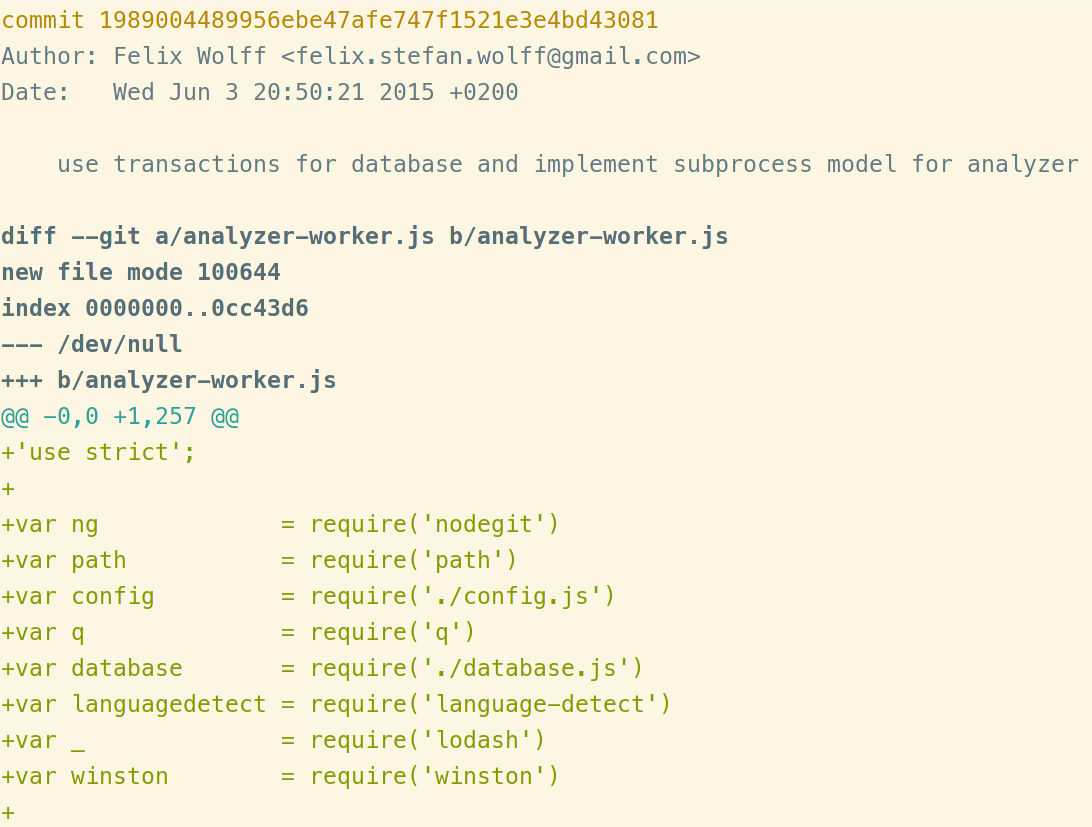
\includegraphics[width=30em]{gfx/commit.png}
    \caption{A sample commit displaying all of the relevant data: date, author with e-mail, diff}
    \label{fig:commit}
\end{figure}

\section{Existing software sizing methods}
Estimating software development effort came up as early as 1981, when Barry W. Boehm invented the \textit{Constructive Cost Model} (COCOMO)\footnote{\url{http://en.wikipedia.org/wiki/COCOMO} | checked June 10, 2015}.
It is a simple measure for estimating code cost based on two main factors: developer count and development time.
\newline

It assumes that more developers will take \textit{less} time to produce the same amount of code, measured in SLOCS\footnote{SLOCS is an abbreviation for \textit{source lines of code}}. This leads to the assumption that more developers produce more code. The project itself does not grow, and thus more developers will finish it faster - a dangerously wrong assumption of historical importance\cite{fb:1975}.
\newline

Research on other measurement methods clearly shows that measuring function points\footnote{\url{http://bit.ly/1C1yys5} | checked June 10, 2015}\footnote{\url{http://bit.ly/1CEmDLy} | checked June 10, 2015} is state-of-the-art for measuring software size and complexity\cite{linkedin:functionpointstandard}. A function point is the unit of measurement that expresses the amount of business functionality a system provides to a user. This is a wholistic measure, meaning that it analyzes the code as-is and does not take into account individual contributions.

Clearly, measuring function points brings comparably better results than counting SLOCs as it is programming language-agnostic and measures the value of user-relevant program features, which makes it more business-relevant. As a side note, counting SLOCs remains present in many companies as processes have been formed around it. Some companies even resorted to paying bonuses for higher line counts\cite{am:2009}.
\newline

Measuring wholistic development effort that has gone into a project as a whole\footnote{\url{http://www.locmetrics.com/alternatives.html} | checked June 10, 2015} is not the approach we need, because it does not take historical data from version control systems into account and makes no distinction between individual contributions.

\section{A custom metric}
This section deals with constructing a metric for answering the research question from \ref{subsec:dev-skill-measurement}. We decided to construct a new metric for this. Most large-scale projects make use of more than one programming language or technology\footnote{see \eg the \href{http://projects.apache.org/indexes/language.html}{Apache Software Foundation Programming Language Index}}, which is why language-sensitivity needs to be part of our metric. The analyzed job offers ask for a minimum experience level with a certain technology, which is why it should consider the experience level as well.

\subsection{A naive approach}
The data available to us consisted strictly out of commits and code statistics. Two assumptions were as follows:

\begin{itemize}
 \item The more experienced a developer, the more code he has seen and written. This experience maps to a timespan worth of work with this technology.
 \item Every human being is different, and as such, developers might have different learning paces. To attribute these, it makes sense to have experience as an abstract measure. This allows the metric to rank fast learners and slow learners on the same level, where the slow learner simply had more time.
\end{itemize}

Unfortunately, the only measurement we were able to make is the number of lines written. As outlined in the previous chapter, measuring SLOC is widely regarded as a bad practice beacause it simply cannot be determined whether the writing of a single line has taken ten seconds or five hours. And again, the kind of language used plays a huge role. On the one hand, a single line of ASM does take less time to write than a single line in JavaScript and will have very little effect on data in main memory. On the other hand, the line in ASM is much harder to write, because the whole memory structure needs to be understood. The answer which line is worth more in this case is very hard to answer. It is dependant on lots of factors - some of which are measurable and some of which are soft. Unfortunately, there is not a lot of research available on the topic of line-based measurements. Many opinionated articles exist\footnote{\url{http://bit.ly/1BRku4a} | checked June 29, 2015}\footnote{\url{http://bit.ly/1BRkAso} | checked June 29, 2015}\footnote{\url{http://bit.ly/1GVzugg} | checked June 29, 2015}, which was evidence enough for us that this approach should be avoided.

\subsection{Technical fit}\label{sec:technicalfit}
From the data that each commit sports it is possible to say when a developer used a programming language for the first time in a project. By aggregating the data over several repositories, it is possible to say when he has used it for the first time in general on GitHub. This resolution of experience is based on timestamps and not on SLOC, which has the disadvantage of being not accessible for fast learners but relieves us of the neccessity to define a mapping of SLOC to a timespan. By using the first and last dates for commits that were made with a certain language, the timespan of experience with this language can easily be calculated, like in formula \ref{eq:timespan}.

\begin{align}
\begin{split}\label{eq:timespan}
timespan(language) ={}& date(lastcommit(language)) - \\
                      & date(firstcommit(language))
\end{split}
\end{align}

This simple calculation alone bears the fallacy that people who use a programming language rarely but every few years get attributed lots of experience. This is solved by the introduction of a \textit{productivity parameter}, which is based off the number of commits one makes per day - as formula \ref{eq:productivity} shows.

\begin{equation}
productivity(language) = \frac{numberofcommits(language)}{timespan(language)}
\label{eq:productivity}
\end{equation}

There is a downside to this, however. It rewards people who commit large files of source code they have not written. A good example might be a commit that contains the \textit{node\_modules} library folder from a Node.js project. In a single commit, this developer will have been attributed thousands of lines of JavaScript.

Small commits are preferred \cite{so:commitsize} over very large commits as they provide a better level of granularity for reverting\footnote{git revert} or cherry-picking\footnote{git cherry-pick}. For this reason, they have become more or less of a standard in free  open source software projects, with 50\% percent of all commits being reasonably small\cite{rsk:2014}. With this in mind, it makes sense to introduce another factor into the metric that gives credit to developers who make small commits, allowing for better teamplay:

\begin{equation}
averageCommitSize(language) = \frac{\sum_{c \in commits(language)} lines(c)}{count(commits)}
\label {eq:avgcommitsize}
\end{equation}

Ranking by the three values, the developers best suited for a position \textit{from the technical perspective} are the ones who have the \textit{greatest timespans}, the \textit{highest productivity}, but the \textit{lowest averageCommitSize}. This metric tries only to capture experience with programming languages, and not experience with technologies.

\subsection{Cultural fit}
Technical competencies aside, nobody wants to work with someone who does not "fit in". A technical fit does not guarantee such a cultural fit. GitHub provides precious little data for gaining insight into the personality of a user.
\newline

A small indicator about the poularity of someone might be the way his profile is valued. On GitHub, users can follow each other and be notified of the actions of their followings. The value of these counters might be a hint of importance and social acceptance.
\newline

GitHub used to provide users with the possibility to write about themselves. Their API still provides a way to read this short biography\footnote{\url{https://developer.github.com/v3/users/} | checked June 29, 2015}, but that is unfortunately a remnant of its removal. This data will be removed in a future version, which was confirmed upon request (see figure \ref{fig:gapitweet}). Some ideas to gain insight into candidate personality are outlined in section \ref{sec:future-work}.

\begin{figure}
  \centering
  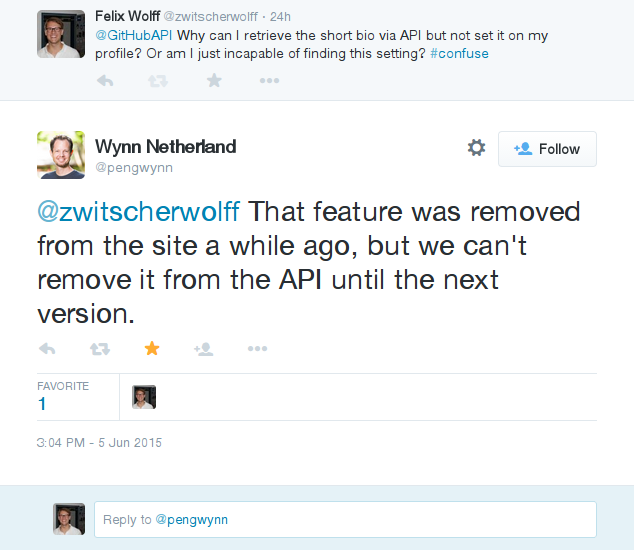
\includegraphics[width=25em]{gfx/githubapi_tweet.png}
  \caption{The tweet that confirmed that the \textit{bio} field is scheduled for removal}
  \label{fig:gapitweet}
\end{figure}

\section{Downsides}\label{sec:threatstovalidity}
For the metric to deliver meaningful results, the base data
needs to be sufficiently large and all e-mail addresses that were used for
making commits need to be registered with the GitHub profile.

Someone who used a open-source component at work, made a small bugfix,
and contributed it back into the project, but left his profile untouched
since then, will not have a very good standing because the data
for attaing one is simply missing. He may even be a very good developer
but any work not published to GitHub will not be considered.
%************************************************
\chapter{Implementation}\label{ch:implementation}
%************************************************
In order to verify the metric, an application that appealed both to developers as well as employers needed to be built. It should motivate developers to grant it access to their public repositories, and convince recruiters to use it. The special means that the development of the application required will be described in this chapter.

\section{Architecture}
Web applications are state-of-the art as they require little servicing and no complex versioning. Our use case of many users taking advantage of a common dataset is perfect for this architecture. We decided to implement the serverside logic in Node.js, which is a JavaScript runtime. The client-side runs in the browser and makes use of standard web technologies like CSS3, HTML5 and JavaScript. The analysis results are saved in a SQLITE3 database.
\newline

The serverside part needs to master two tasks: serving data to clients as well as analyzing repositories from developers. These are two very different concerns. In order not to stall one of the tasks while executing the other, we decided to have two dedicated processes running alongside each other. One of these will serve the data and perform queries on the database, while the other will keep the local copies of the repositories up to date and build the metric on them. We will call the first component the \textit{hirebot} and the latter the \textit{analyzer}.

\subsection{Database schema}
The database schema of hirebot is not very complex. Users are central to the application and every other type of data is associated with one, as seen in figure \ref{fig:schema}. Basic data retrieved from the GitHub API is saved as well as the values generated from the repositories.

\begin{figure}
  \centering
  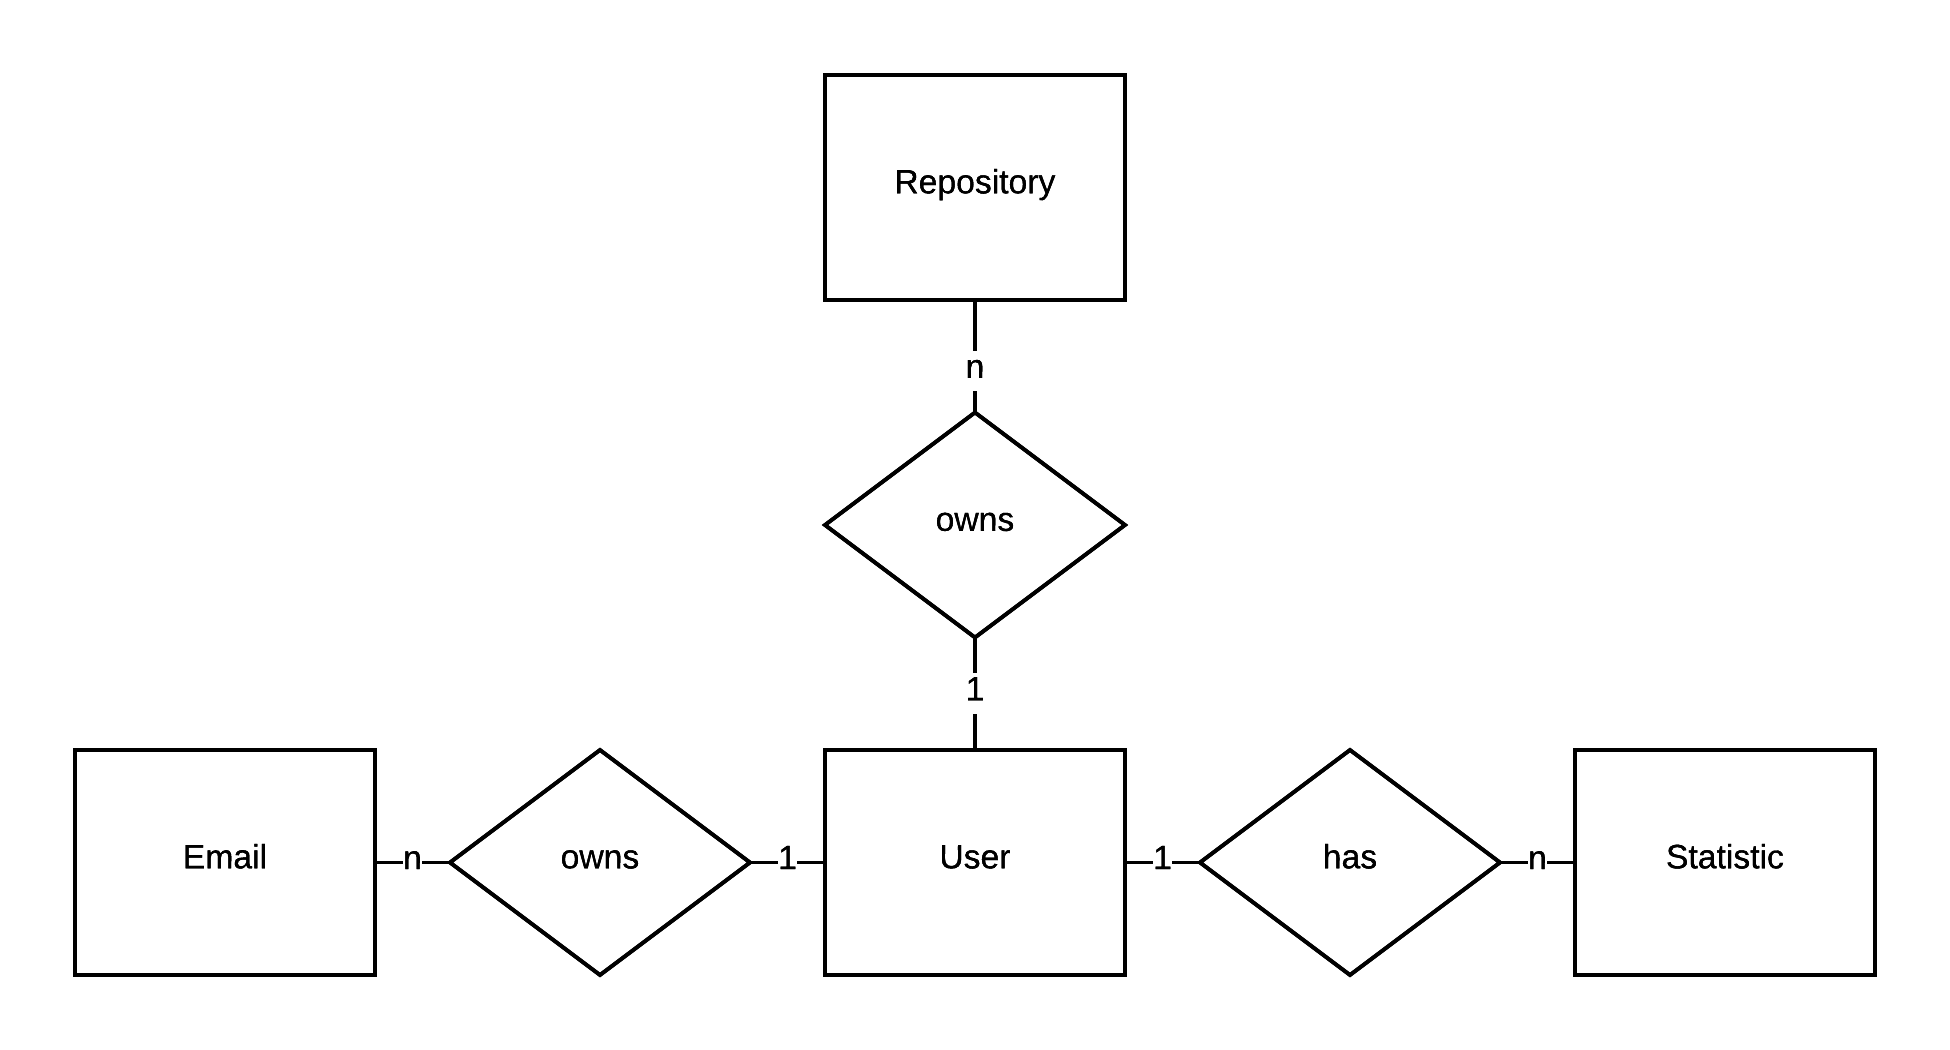
\includegraphics[width=35em]{gfx/schema.png}
  \caption{The hirebot database schema. Only attributes that are mined from the code are listed. To preserve space, attributes are grouped in curly braces if they share prefixes or suffixes}
  \label{fig:schema}
\end{figure}

\subsection{Hirebot}
The component playing the webserver role is called \textit{hirebot}. It handles the usual webserver tasks like formatting templates and querying the database for answering HTTP requests to an endpoint.
\newline

Additionally, it implements the foundation for data analysis. It allows developers to register with GitHub to grant the application access to their email addresses and their repositories. Hirebot then notifies the analyzer, which continues with cloning and analyzing the repositories. This process is also depicted in figure \ref{fig:regprocess}.

\begin{figure}
  \centering
  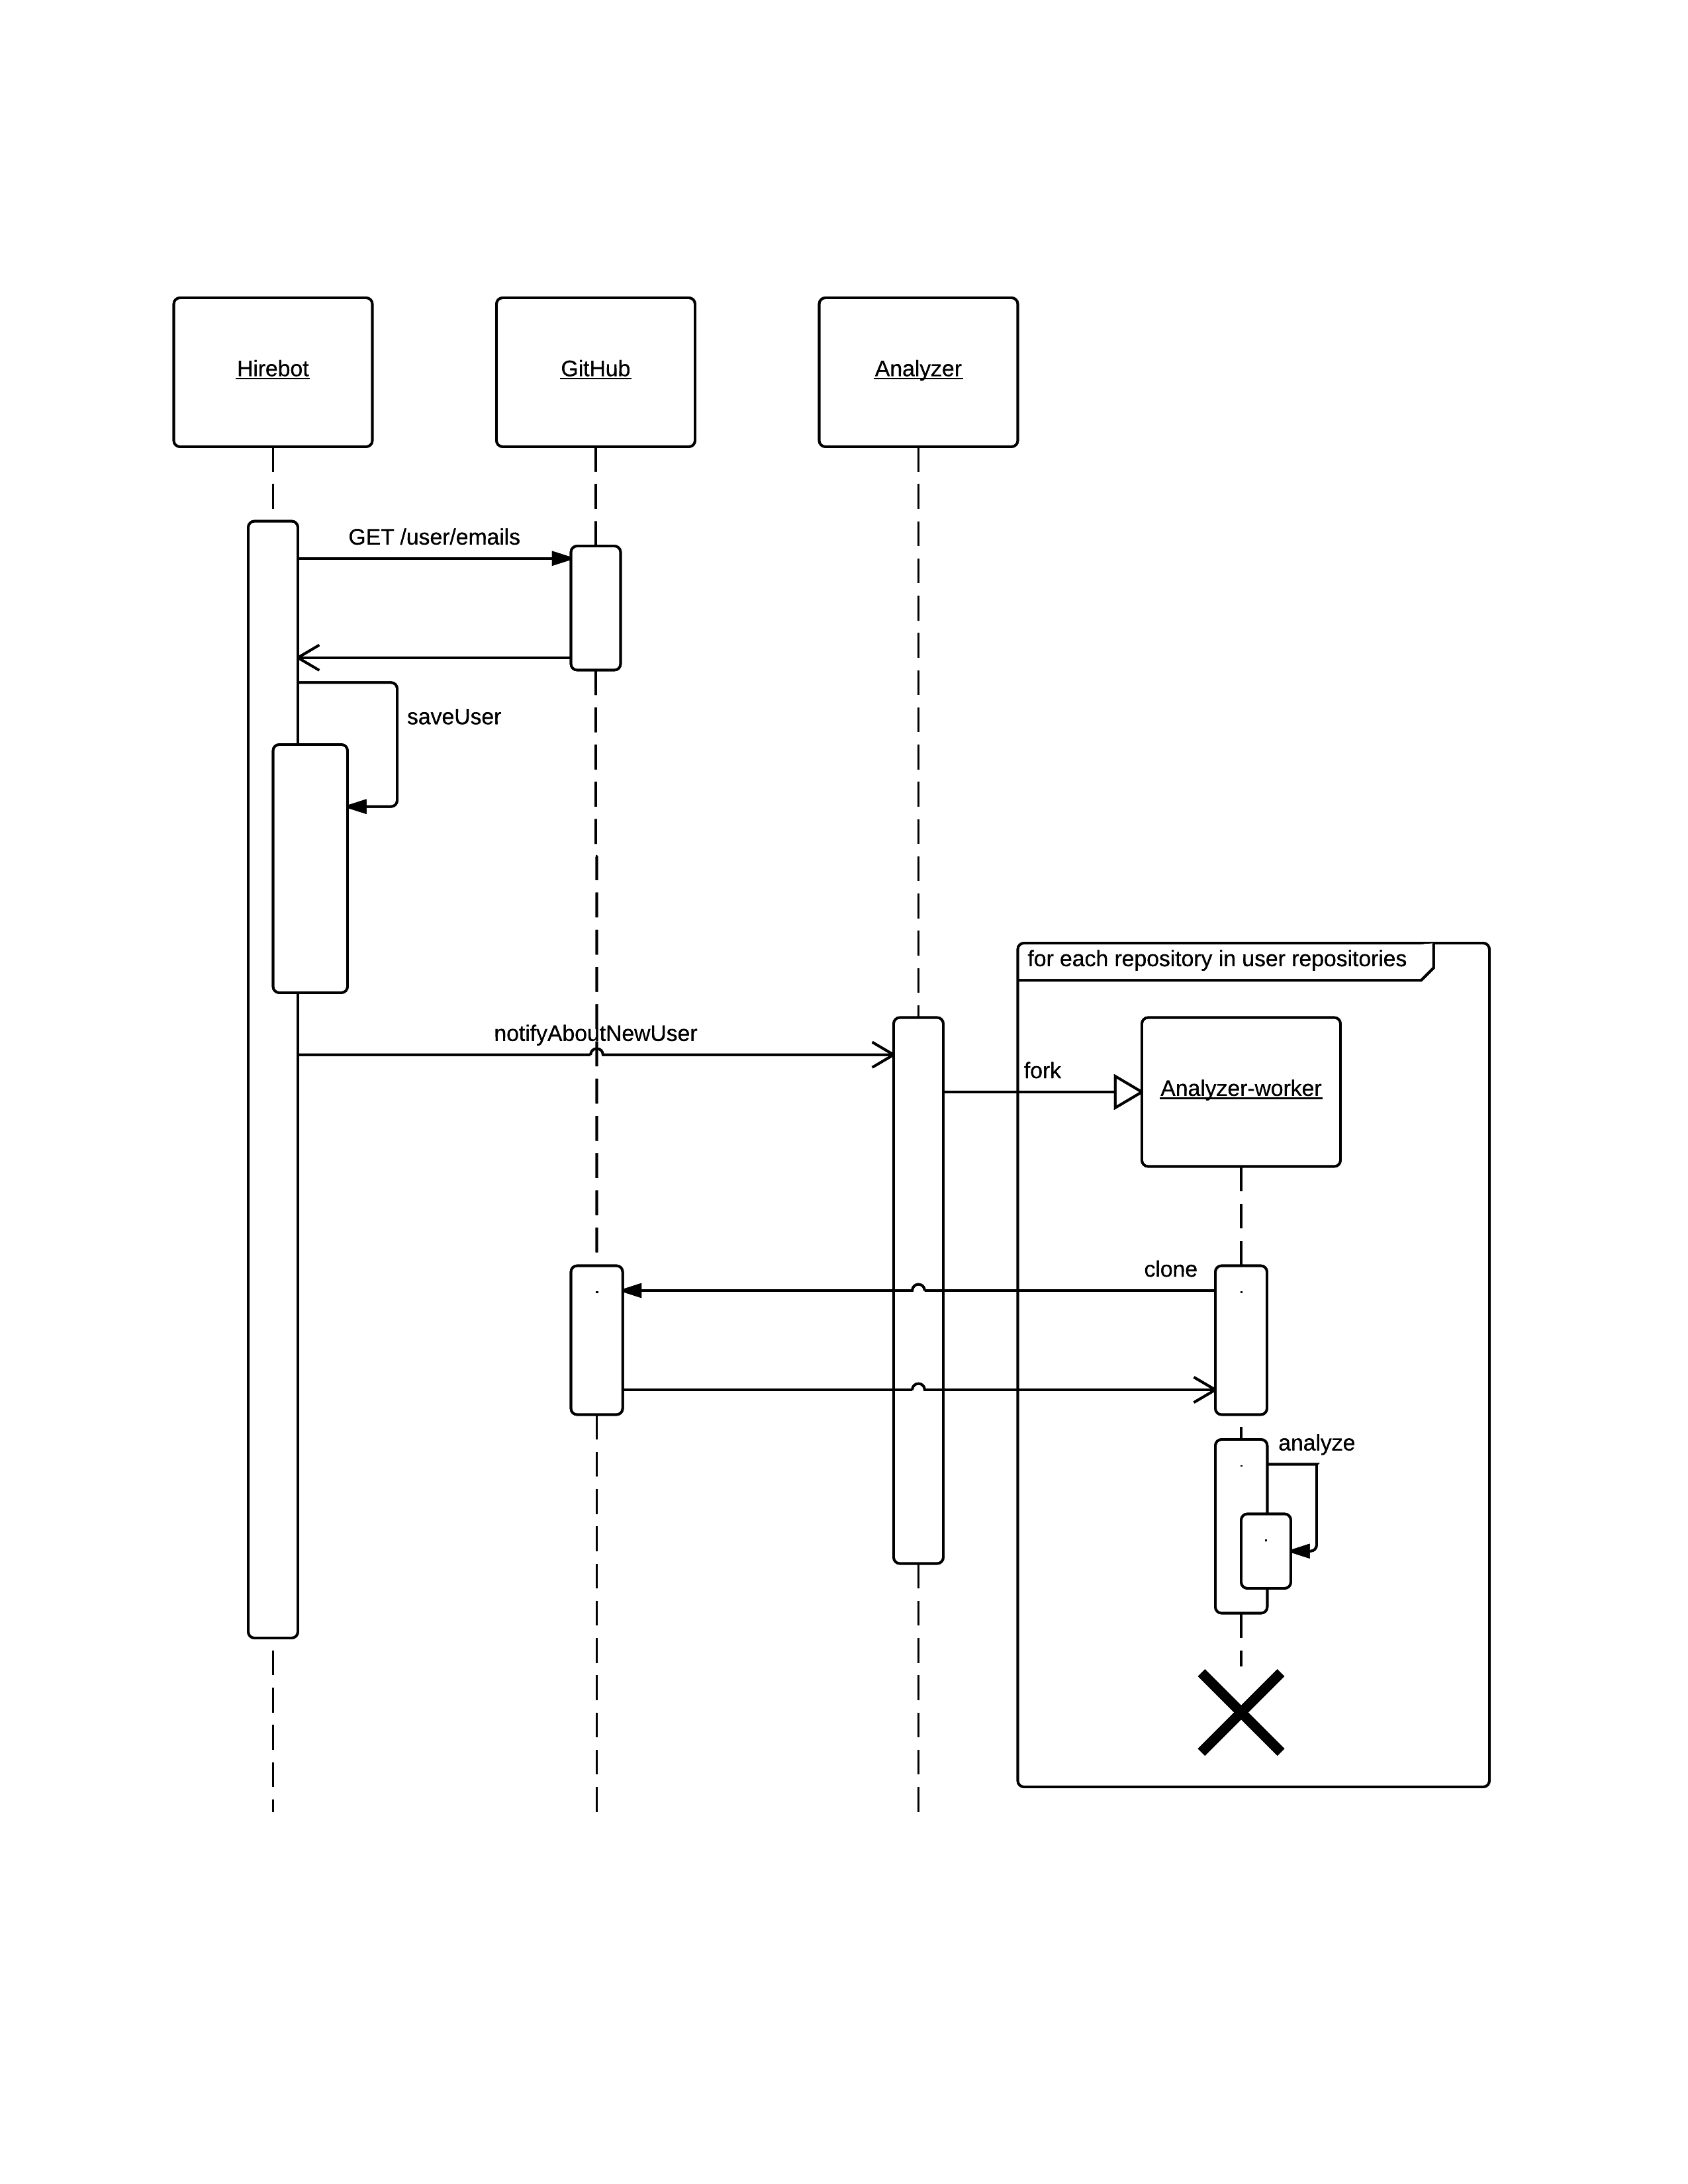
\includegraphics[width=35em]{gfx/registersequence.png}
  \caption{The interplay of the three processes with the GitHub API after the OAuth 2.0 dance has been completed.}
  \label{fig:regprocess}
\end{figure}

\subsection{Analyzer}
The analyzer component of the application handles two slightly different tasks. First, it has to schedule an initial clone of all repositories a user owns upon his registration. Then, it has to keep those local copies up to date and add new repositories, both in a recurring fashion.


\textit{Nodegit}, the library that was used for accessing the git repository data, was leaking memory strongly causing resource problems. To counter this, a sub-process structure was implemented. The analyzer itself only executes management logic, schedules the analysis, and communicates with the hirebot process. For executing the analysis, it forks an \textit{analyzer-worker} for each single repository. The worker clones or updates that repository, runs the analysis, saves the results into the database and terminates upon completion. The forks are done sequentially to avoid putting too much load on the system at once.

\subsection{Metric implementation}\label{sec:metric-implementation}
The metric described in section \ref{sec:technicalfit} is fully implemented in the analyzer-worker component. Its implementation works on a repository basis and can be illustrated with the following pseudo-code down like this:\\[.25em]

\begin{algorithmic}
\For{c:=mostRecentlyAnalyzedCommit to lastCommit}
  \For{d:= c.firstDiff to c.lastDiff}
    \State language = determineFileLanguage(d.file)
    \State lineCount = d.lineCount
    \State saveExperience(language, c.id, c.date, lineCount)
  \EndFor
\EndFor
\end{algorithmic}
\vspace{0.75em}

Additionally, a special JavaScript analyzer was built into the algorithm. It adds McCabe\cite{mc:1976} and Halstead\cite{h:1977} complexity metric information about single commits. Thus, the final implementation amounts to:\\[.25em]

\begin{minipage}{\linewidth}
\begin{algorithmic}
\For{c:=mostRecentlyAnalyzedCommit to lastCommit}
  \For{d:= c.firstDiff to c.lastDiff}
    \State language = determineFileLanguage(d.file)
    \State lineCount = d.lineCount
    \State saveExperience(language, lineCount)
    \State
    \If{language = JavaScript}
      \State fileContentsBeforeCommit = d.file.contents
      \State fileContentsAfterCommit  = d.parent.file.content

      \State mcB = mcCabeComplexity(fileContentsBeforeCommit)
      \State mcA = mcCabeComplexity(fileContentsAfterCommit)
      \State hB = halsteadComplexity(fileContentsBeforeCommit)
      \State hA = halsteadComplexity(fileContentsAfterCommit)
      \State
      \State saveJavaScriptMeasures(c.id, c.date, mcB, mcA, hB, hA)
    \EndIf
  \EndFor
\EndFor
\end{algorithmic}
\end{minipage}
\vspace{0.75em}

Even though the extra JavaScript metrics above are not considered in the final evaluation of our metric, they serve as an example of how to gain insights into per-commit changes of overall complexity and size, like it has been done extensibly in Gieses' work\cite{pg:2014}.

\subsection{Metric evaluation}
The metric is aggregated from the raw commit analysis data using an SQL view called \verb=calculatedmetric=.

\marginpar{A view allows us to use aggregated data without requring extra work with an additional table.}

%\begin{lstlisting}[language=SQL, frame=false]
%CREATE VIEW IF NOT EXISTS calculatedmetric AS
%  SELECT userid, language, MIN(date) AS firstcommitdate,
%    MAX(date) AS lastcommitdate, SUM(lines) AS linecount,
%    COUNT(commitid) AS commitcount,
%    julianday(MAX(date))-julianday(MIN(date)) AS timespan,
%    SUM(lines)/COUNT(commitid) AS averagecommitsize,
%    (julianday(MAX(date)) - julianday(MIN(date)))/COUNT(commitid)
%      AS productivity
%  FROM statistics GROUP BY userid, language
%  HAVING MIN(date) <> MAX(date)
%  ORDER BY userid, timespan DESC, productivity ASC
%\end{lstlisting}

Upon querying candidates who suit certain requirement levels, a little logic becomes necessary to build the query. To include candidates in the result set who can provide \textit{some} of the skills, it is necessary to construct combinations of the required programming languages. I.e. if Java, C++ and JavaScript experience levels of at least 3 years were asked for, there would be four combinations, not counting the single options. Thus, four queries need to be built and executed:

\begin{itemize}
  \item Java \textit{AND} C++ \textit{AND} JavaScript
  \item Java \textit{AND} C++ \textit{AND NOT} JavaScript
  \item C++ \textit{AND} JavaScript \textit{AND NOT} Java
  \item JavaScript \textit{AND} Java \textit{AND NOT} C++
\end{itemize}

%\begin{minipage}{\linewidth}
%\begin{lstlisting}[language=SQL, frame=false]
%SELECT id, profilename, name, profileurl, avatarurl, location, hireable, followers, following FROM users u
%  WHERE 'Java' IN (SELECT language FROM calculatedmetric WHERE userid = u.id AND timespan >= 360*1.5)
%    AND 'C++' IN (SELECT language FROM calculatedmetric WHERE userid = u.id AND timespan >= 360*1.5)
%    AND 'JavaScript' IN (SELECT language FROM calculatedmetric WHERE userid = u.id AND timespan >= 360*1.5)
%
%SELECT id, profilename, name, profileurl, avatarurl, location, hireable, followers, following FROM users u
%  WHERE 'Java' IN (SELECT language FROM calculatedmetric WHERE userid = u.id AND timespan >= 360*1.5)
%    AND 'C++' IN (SELECT language FROM calculatedmetric WHERE userid = u.id AND timespan >= 360*1.5)
%    AND NOT 'JavaScript' IN (SELECT language FROM calculatedmetric WHERE userid = u.id AND timespan >= 360*1.5)
%...
%\end{lstlisting}
%\end{minipage}

\section{Interface}
\subsection{Candidate view}
A candidate can view his general personal statistics and the JavaScript statistics mentioned above. This provides him with insight about what job offers he might receive and what to improve about his coding style (see figure \ref{fig:candidateview}).

\begin{figure}
  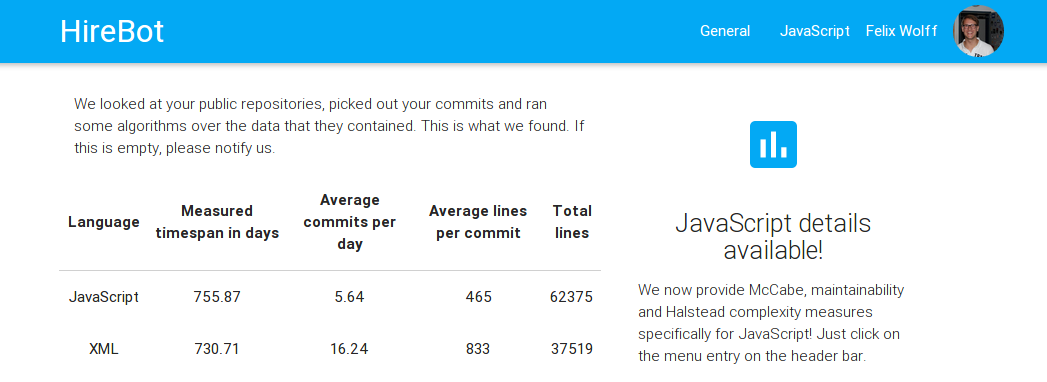
\includegraphics[width=30em]{gfx/candidateview.png}
  \caption{The candidate view of Hirebot}
  \label{fig:candidateview}
\end{figure}

\subsection{Employer view}
In a small search form, a recruiter can state his requirements concerning programming language knowledge and for how long this skill should be in posession (see figure \ref{fig:employerview}).

%************************************************
\chapter{verification}\label{ch:verification}
%************************************************
The whole purpose of the implementation was acquiring real data for finding an answer to research question 2 from section \ref{subsec:measurement-quality}. We did so by conducting a series of short interviews. Most users who registered with the application during the testing phase were HPI students, so finding partners for interviews did not prove a great difficulty.

\section{Interviews}\label{sec:interviews}
The objective of each interview was to verify how the interviewee personally viewed his suitability for a certain position. Finding out about personal interest in the position is not a goal. Interviewees should try to apply a metric similar to ours, i.e. based on their technical abilities. Afterwards their answers were compared to the recommendations made by the algorithm.

Three candidates were chosen by looking at the ranking results generated by Hirebot. The job openings were chosen in such a way that they required different skills, and the ranking produced different results. The candidates were interviewed individually. They were given the technical requirement summaries of 4 job openings on small cards and should make statements about their suitability for them. Afterwards, they were shown the real job offering, complete with the introductory text. Any deviations from their previous statements were noted. Afterwards, the suitabilities expressed by the candidates were compared to the suitabilities determined with our metric.

In the following, job opening shall be abbreviated with JO.

\subsection{Reference job openings}
We used four job openings from four very different institutions, two small startups, a university and a huge established corporation. All of them can be viewed in their entireity in the Appendix \ref{chap:appendix}. They were summarized as follows:

\begin{enumerate}
\item Two years of Python, Knowledge of Java/C++ and SQL.
\item Three years of Ruby and 3 years of JavaScript
\item Five years of C++
\item One year of HTML, JavaScript and CSS
\end{enumerate}

\subsection{Interview 1}
``Not a perfect match, but nonetheless interesting because of Java and C++ or Ruby" were the words spoken in reaction to seeing the summaries to JO1 and JO2. JO3 was also not called a good match, because not the full five years worth of experience with C++ could be provided. JO4 was titled a ``perfect fit".\\
These opinions also did not change greatly upon viewing the whole job opening descriptions, except for JO3. Upon reading the whole description, he strongly argumented against this position for he knew nothing of astrology and did not want to work in the academic field. He mentioned that the programming language requirements were generally helpful at a glimpse but he would have wished for technology requirements and a short description of the work environment.

\subsection{Interview 2}
JO1 was declared a bad fit, because he only knew some of the programming languages required, specifically not Python. Upon reading the whole job offer however, he announced that he could do it because he could learn Python quickly. This no-then-yes-pattern was repeated with JO2. At first the job was called a bad fit because of the required proficiency in Ruby. After reading the whole posting, where the neccessity of this was verbally reduced and some used technologies like AngularJS were mentioned, he repositioned himself with a clear approval. JO3 was rejected both times because of lack of skill, and JO4 was accepted both times because the required skills could easily be provided.

\subsection{Interview 3}
This candidate was positive about almost every job offer. JO1 was called a good match. JO2 was turned down, because his experience in both Ruby and JavaScript was not very advanced. JO3 und JO4 were partial fits, because there he did not have a lot to show for C++ or web frontend development. This attitude did not change after going through the whole text of each offering. He also mentioned that while Node.js was technically JavaScript, he would have liked the summary to mention it, because he saw a strong distinction between JavaScript used in frontend and backend.

\section{Key findings}\label{sec:key-findings}
All candidates stated that they were equally interested in technologies as well as programming language requirements. Also, interview partner 1 stated to have capabilities in C++. These were not tracked because he did not have any repositories on GitHub which contained source code written in that language. Another caveat that was described as unwanted was the suggestion of a job in academia. Both of the issues mentioned can be addressed via means that are described in more detail in section \ref{sec:future-work}.

\section{Candidate fit}
As outlined in section \ref{sec:interviews}, the interviewees were chosen with their ranking known. A comparison of where the ranking displayed a total fit and where the candidates saw themselves fit can be seen in table~\ref{table:rank-comparison}.

\begin{table}
\centering
\begin{tabular}{c|cccc}
Candidate \# & JO1 & JO2 & JO3 & JO4\\
\hline
           1 & & $\frac{1}{2}$C & & C|$\frac{2}{3}$R\\
           2 & & $\frac{1}{2}$C|R & & C|R\\
           3 & C|R & $\frac{1}{2}C$|$\frac{1}{2}R$ & C & \\
\end{tabular}
\caption{A comparison of ranking results and the candidates own opinions, because candidates should know their own suitability for a job best. An R marks ranking fit, and a prefixed fraction marks partial fit. The same goes for C, demarking candidate opinion.}
\label{table:rank-comparison}
\end{table}

The ranking matched candidate opinion almost every time. Given the fact that the candidates had very rich GitHub profiles sporting an average of 23 repositories, our metric seems to work reasonably well if enough data is supplied. A minimum repository count of 10 seems to work out fine\footnote{This value has been determined in a series of small experiments and will probably be subject to change.}. Possibilities on how to improve the ranking are outlined in the following and last section. Nonetheless we conclude that the answer to the second research question is a clear yes. Our metric is a good step into the direction of candidate identification.
%************************************************
\chapter{Conclusion}\label{ch:conclusion}
%************************************************
\section{Future work}\label{sec:future-work}
The Hirebot platform is a very basic prototype and extensible in many directions. In the following, improvements that might improve usability and ranking are described.

An account on GitHub is certainly very promising, but it is not the only place where one can publish code. There are similar services like Gitorious, Bitbucket or GitLab and of course self-hosted git-repositories. If one has made significant contributions to these codebases, these will not show up in the final statistics, as outlined in section \ref{sec:threatstovalidity} and criticized in section \ref{sec:key-findings}. As such, it should at least be possible to manually add other repositories by hand, or connect other platforms in a process similar to that used with GitHub.

The connection with other platforms leads to another possible improvement that might cancel out false recommendations, also a critic picked up during the interviews. Instead of relying on a single source, it would make very much sense to pull in information from others to improve the basis for decision. There are numerous job profile sites like XING\footnote{\url{http://xing.de} | checked June 10, 2015} or LinkedIn\footnote{\url{http://linkedin.com} | checked June 10, 2015} where users have published their complete curriculum vitaes. A profile here can hint at the suitability of a candidate for a position. For example a user that is found to be suitable for a data engineer position might not want to leave his job at a technology consultancy firm - he is just developing in his own interest. While it is possible to indicate availability by using the hireable flag (see section \ref{sec:data-source}), very many GitHub users do not use this feature, making external data necessary. Other interesting sources include Openhub\footnote{\url{http://openhub.net} | checked June 10, 2015} and Stackoverflow\footnote{\url{http://stackoverflow.com} | checked June 10, 2015}. By using the techniques for identifying developers across StackOverflow and GitHub\cite{vfs:2012}, it could be possible to enrich user profiles automatically to better identify personal topic preferences. With this information at hand, building something similar to a Klout score\footnote{\url{http://mashable.com/2011/06/29/work-for-pie} | checked June 10, 2015}. is possible

The reliable identification of candidates across several sources also rids the system of the necessity of registrations. Developers can easily be \textit{found} by crawling the GitHub API, thus increasing the userbase for recommendations.


Lots of job advertisements also put emphasis on certain technologies. For instance it does not suffice to know JavaScript - specifically AngularJS (a client-side JavaScript framework) needs to be well known for at least three years. With the current state of development this kind of differentiation is not possible. No distinctions between front-end or backend code are made, nor are specific technologies considered. This would require technology-specific context and a complex distinction logic as the lines between frontend and backend code begin to blur. For example, Node.js backend-code can easily be run in any web browser using browserify\footnote{\url{http://browserify.org} | checked June 10, 2015}.
\newline

To improve the metric, it makes sense to analyze code sections before and after the commit for changes in complexity and other quality measures. As shown by Giese \cite{pg:2014} and in section \ref{sec:metric-implementation}, this is just another step in the analysis process. Now, if a developer strives to reduce complexity with his commits, this can be rewarded with a boost in the overall ranking. Likewise, complexity-increasing commits should be punished. Once more languages than JavaScript are covered, this seems a worthwhile investment of development effort: employers get into contact with highly skilled developers while students who are good at coding can move up the ranks.

\section{Conclusion}
In this thesis we have constructed a metric as an approach to measuring developer skill. Even though Yashamita et al. claim that software metrics alone can not be used to assess source code\cite{mlya:2012}, it is possible to use these metrics to match code authors to job opening skill requirements by comparing provided and demanded skills. At the heart of research lies Hirebot, a platform where developers can sign up with their GitHub account. Upon registration their public repositories are cloned and data to construct the metric on is gathered. Developers can view their own statistics to get a feeling for what programming languages they have provided data and recruiters can easily enter programming language requirements and receive candidate suggestions. Hirebot was built specifically to verify our metric with real data. As demonstrated in the previous chapter, the results are acceptably good for the amount of data gathered, and we are confident to have found a good solution to the problem.

Having demonstrated the feasibility of an algorithmic matching approach of developers to technical job openings, we believe that it is only a question of time and effort until anyone can be matched on to any job opening automatically.
%The rankings will take into account more and more data, perhaps even checking for a cultural or personality fit.
% ********************************************************************
% Backmatter
%*******************************************************
\appendix
%\cleardoublepage
\part{Appendix}
%%********************************************************************
%% Appendix
%%*******************************************************
%% If problems with the headers: get headings in appendix etc. right
%%\markboth{\spacedlowsmallcaps{Appendix}}{\spacedlowsmallcaps{Appendix}}
%\chapter{Appendix Test}
%Lorem ipsum at nusquam appellantur his, ut eos erant homero
%concludaturque. Albucius appellantur deterruisset id eam, vivendum
%partiendo dissentiet ei ius. Vis melius facilisis ea, sea id convenire
%referrentur, takimata adolescens ex duo. Ei harum argumentum per. Eam
%vidit exerci appetere ad, ut vel zzril intellegam interpretaris.
%
%Errem omnium ea per, pro congue populo ornatus cu, ex qui dicant
%nemore melius. No pri diam iriure euismod. Graecis eleifend
%appellantur quo id. Id corpora inimicus nam, facer nonummy ne pro,
%kasd repudiandae ei mei. Mea menandri mediocrem dissentiet cu, ex
%nominati imperdiet nec, sea odio duis vocent ei. Tempor everti
%appareat cu ius, ridens audiam an qui, aliquid admodum conceptam ne
%qui. Vis ea melius nostrum, mel alienum euripidis eu.
%
%\section{Appendix Section Test}
%Ei choro aeterno antiopam mea, labitur bonorum pri no. His no decore
%nemore graecis. In eos meis nominavi, liber soluta vim cu. Sea commune
%suavitate interpretaris eu, vix eu libris efficiantur.
%
%\graffito{More dummy text.}
%Nulla fastidii ea ius, exerci suscipit instructior te nam, in ullum
%postulant quo. Congue quaestio philosophia his at, sea odio autem
%vulputate ex. Cu usu mucius iisque voluptua. Sit maiorum propriae at,
%ea cum primis intellegat. Hinc cotidieque reprehendunt eu nec. Autem
%timeam deleniti usu id, in nec nibh altera.
%
%\section{Another Appendix Section Test}
%Equidem detraxit cu nam, vix eu delenit periculis. Eos ut vero
%constituto, no vidit propriae complectitur sea. Diceret nonummy in
%has, no qui eligendi recteque consetetur. Mel eu dictas suscipiantur,
%et sed placerat oporteat. At ipsum electram mei, ad aeque atomorum
%mea.
%
%\begin{table}
%    \myfloatalign
%  \begin{tabularx}{\textwidth}{Xll} \toprule
%    \tableheadline{labitur bonorum pri no} & \tableheadline{que vista}
%    & \tableheadline{human} \\ \midrule
%    fastidii ea ius & germano &  demonstratea \\
%    suscipit instructior & titulo & personas \\
%    %postulant quo & westeuropee & sanctificatec \\
%    \midrule
%    quaestio philosophia & facto & demonstrated \\
%    %autem vulputate ex & parola & romanic \\
%    %usu mucius iisque & studio & sanctificatef \\
%    \bottomrule
%  \end{tabularx}
%  \caption[Autem usu id]{Autem usu id.}
%  \label{tab:moreexample}
%\end{table}
%
%Ei solet nemore consectetuer nam. Ad eam porro impetus, te choro omnes
%evertitur mel. Molestie conclusionemque vel at, no qui omittam
%expetenda efficiendi. Eu quo nobis offendit, verterem scriptorem ne
%vix.
%
%
%\begin{lstlisting}[float,caption=A floating example]
%for i:=maxint to 0 do
%begin
%{ do nothing }
%end;
%\end{lstlisting}
%********************************************************************
% Other Stuff in the Back
%*******************************************************
\cleardoublepage%********************************************************************
% Bibliography
%*******************************************************
% work-around to have small caps also here in the headline
\manualmark
\markboth{\spacedlowsmallcaps{\bibname}}{\spacedlowsmallcaps{\bibname}} % work-around to have small caps also
%\phantomsection 
\refstepcounter{dummy}
\addtocontents{toc}{\protect\vspace{\beforebibskip}} % to have the bib a bit from the rest in the toc
\addcontentsline{toc}{chapter}{\tocEntry{\bibname}}
\bibliographystyle{plainnat}
\label{app:bibliography} 
\bibliography{Bibliography}
%\cleardoublepage\pagestyle{empty}

\hfill

\vfill


\pdfbookmark[0]{Colophon}{colophon}
\section*{Colophon}
This document was typeset using the typographical look-and-feel \texttt{classicthesis} developed by André Miede.
The style was inspired by Robert Bringhurst's seminal book on typography ``\emph{The Elements of Typographic Style}''.
\texttt{classicthesis} is available for both \LaTeX\ and \mLyX:
\begin{center}
\url{http://code.google.com/p/classicthesis/}
\end{center}
Happy users of \texttt{classicthesis} usually send a real postcard to the author, a collection of postcards received so far is featured here:
\begin{center}
\url{http://postcards.miede.de/}
\end{center}

\bigskip

\noindent\finalVersionString

%Hermann Zapf's \emph{Palatino} and \emph{Euler} type faces (Type~1 PostScript fonts \emph{URW
%Palladio L} and \emph{FPL}) are used. The ``typewriter'' text is typeset in \emph{Bera Mono},
%originally developed by Bitstream, Inc. as ``Bitstream Vera''. (Type~1 PostScript fonts were made
%available by Malte Rosenau and
%Ulrich Dirr.)

%\paragraph{note:} The custom size of the textblock was calculated
%using the directions given by Mr. Bringhurst (pages 26--29 and
%175/176). 10~pt Palatino needs  133.21~pt for the string
%``abcdefghijklmnopqrstuvwxyz''. This yields a good line length between
%24--26~pc (288--312~pt). Using a ``\emph{double square textblock}''
%with a 1:2 ratio this results in a textblock of 312:624~pt (which
%includes the headline in this design). A good alternative would be the
%``\emph{golden section textblock}'' with a ratio of 1:1.62, here
%312:505.44~pt. For comparison, \texttt{DIV9} of the \texttt{typearea}
%package results in a line length of 389~pt (32.4~pc), which is by far
%too long. However, this information will only be of interest for
%hardcore pseudo-typographers like me.%
%
%To make your own calculations, use the following commands and look up
%the corresponding lengths in the book:
%\begin{verbatim}
%    \settowidth{\abcd}{abcdefghijklmnopqrstuvwxyz}
%    \the\abcd\ % prints the value of the length
%\end{verbatim}
%Please see the file \texttt{classicthesis.sty} for some precalculated
%values for Palatino and Minion.
%
%    \settowidth{\abcd}{abcdefghijklmnopqrstuvwxyz}
%    \the\abcd\ % prints the value of the length





\cleardoublepage%*******************************************************
% Declaration
%*******************************************************
\refstepcounter{dummy}
\pdfbookmark[0]{Declaration Of Authenticity}{Declaration Of Authenticity}
\chapter*{Declaration Of Authenticity}
\thispagestyle{empty}
I certify hereby that the material contained in this document is my own work and
does not contain significant portions of unreferenced or unacknowledged
material. I also warrant that the above statement applies to the implementation
of the project and all associated documentation.\\[1em]

\bigskip

\noindent\textit{\myLocation, \myTime}

\smallskip

\begin{flushright}
    \begin{tabular}{m{5cm}}
        \\ \hline
        \centering\myName \\
    \end{tabular}
\end{flushright}

% ********************************************************************
% Game Over: Restore, Restart, or Quit?
%*******************************************************
\end{document}
% ********************************************************************
